\documentclass[aps,prb,twocolumn,amsmath,superscriptaddress]{revtex4}
\usepackage{graphicx}
\usepackage{color}
\usepackage{epstopdf}
\usepackage{xcolor}
\usepackage{eqnarray,amsmath}

\begin{document}

\title{Resonant photoluminescence and dynamics of coupled hole and Mn spins in a positively charged magnetic quantum dot}


\author{A. Lafuente-Sampietro}
\affiliation{
CNRS, Institut N\'eel, F-38042 Grenoble, France.}
\affiliation{
Universit\'{e} Grenoble Alpes, Institut N\'eel, F-38042 Grenoble, France}

\author{H. Boukari}
\affiliation{
CNRS, Institut N\'eel, F-38042 Grenoble, France.}
\affiliation{
Universit\'{e} Grenoble Alpes, Institut N\'eel, F-38042 Grenoble, France}

\author{L. Besombes}
\email{lucien.besombes@grenoble.cnrs.fr}
\affiliation{
CNRS, Institut N\'eel, F-38042 Grenoble, France.}
\affiliation{
Universit\'{e} Grenoble Alpes, Institut N\'eel, F-38042 Grenoble, France}
\date{\today}

\begin{abstract}

Using resonant optical excitation and resonant photoluminescence, we analyze the initialization efficiency and probe the spin dynamics of an individual magnetic atom (Mn) coupled to a hole spin in a semiconductor quantum dot. A p-doped CdTe/ZnTe quantum dot containing a single Mn atom forms an ensemble of optical $\Lambda$ systems which can be addressed optically. Performing auto-correlation of the resonant photoluminescence intensity and resonant optical pumping experiments we identify the main spin relaxation channels in this multilevel spin system. We evidenced and modelled an efficient spin relaxation mechanism of the coupled hole and Mn spins coming from the interplay of the hole-Mn exchange interaction and the acoustic phonon induced lattice deformation. We show that the $\Lambda$ systems are connected through inefficient forbidden spin-flips than can be enhanced under transverse magnetic field. The dynamics of the resonant photoluminescence in the p-doped magnetic quantum dot is well described by a complete rate equation model.

\end{abstract}

\maketitle

\section{Introduction}

Individual localized spins are promising for the implementation of quantum information technologies in the solid state \cite{Petta2005,Veldhorst2015,Koenrad2011}. Semiconductor quantum dots (QDs) are solid-state systems which permit efficient electrical or optical manipulation of individual carriers spins \cite{Atature2006,Press2008,Gerardot2008,DeGreve2011}. The optical properties of a QD can also be used to control the spin state of individual \cite{Besombes2004,LeGall2011,Kudelski2007,Kobak2014} or pairs \cite{Besombes2012,Krebs2013} of magnetic atoms in transition metal doped semiconductors. The spin of a magnetic atom in a QD can be prepared by the injection of spin polarized carriers and its state can be read through the energy and polarization of the photons emitted by the QD \cite{Besombes2015,Reiter2013,Goryca2009}. The insertion of a magnetic atom in a QD where the charge and strain states can be controlled offers degrees of freedom to tune the properties of the localized spin such as its magnetic anisotropy responsible for the spin memory at zero magnetic field \cite{Oberg2014}.

Positively charged magnetic QDs present a large magnetic anisotropy induced by the exchange interaction between the confined heavy-hole and the localized magnetic atoms spins \cite{Leger2005,Vyborny2012}. Despite the presence of valence band mixing which limits the spin memory, it has been shown that in charge tunable Mn-doped CdTe/ZnTe QDs the hybrid hole-Mn spin can be prepared by optical orientation under excitation with circularly polarized light \cite{Varghese2014}. It was then demonstrated that a positively charged Mn-doped QD forms an ensemble of optical $\Lambda$ systems that can be independently addressed \cite{Lafuente2015} suggesting the possibility to perform coherent manipulation of the magnet formed by the coupled hole and Mn spins with two resonant optical fields \cite{Houel2014}. For an efficient coherent control and a practical use of this hybrid spin in a quantum device one would require however sufficiently long relaxation and coherence times for the two ground hole-Mn states of the $\Lambda$ systems.

In this article, using the resonant photoluminescence (PL) of the positively charged exciton (X$^+$) coupled to a single Mn in charge tunable CdTe/ZnTe QDs \cite{Varghese2014}, we analyze the relaxation mechanisms for the coupled holes and Mn spins. Auto-correlation of the resonant PL and resonant optical pumping experiments reveal an efficient spin relaxation channel of the hole-Mn system: a hole Mn flip-flop induced by the interplay of the hole-Mn exchange interaction and the lattice deformation induced by acoustic phonons. A model predicts hole-Mn flip-flops in the nanosecond range, in agreement with the experiments. We also show that the $\Lambda$ systems are connected by inefficient forbidden spin-flip which are enhanced under a weak transverse magnetic field.

The article is organized as follow: after a description in Sec. II of samples and experiments we shortly present the spin structure of positively charged Mn-doped QDs. In Sec. III we then present the dynamics of the resonant PL probed with auto-correlation measurements. In Sec. IV we discuss resonant optical pumping experiments allowing probing the initialization and relaxation of coupled hole and Mn spins. In Sec. V we present a model describing acoustic phonon induced hole-Mn flip-flops and show that this mechanism is responsible for the large PL observed under resonant excitation. In Sec. VI we model the spin dynamics of positively charged Mn-doped QDs under resonant excitation and compare the calculated autocorrelation curves and optical pumping signal with experimental results.

\section{Samples, experiments and spin structure of a positively charged Mn-doped quantum dot}

The studied sample consists of Mn-doped self-assembled CdTe QDs grown by molecular beam epitaxy on a p-doped ZnTe (001) substrate \cite{Wojnar2011}. A bias voltage can be applied between a semi-transparent 5 nm gold Schottcky gate deposited on the surface of the sample and the p-doped substrate. Under a positive bias, a single hole can be trapped in the magnetic QDs (see figure~\ref{Fig1}(a)) \cite{Varghese2014} and only the emission of the positively charged exciton is observed.

Individual QDs containing one Mn are isolated using micro-spectroscopy techniques \cite{LeGall2010}. A high refractive index hemispherical solid immersion lens is mounted on the surface of the sample to enhance the spatial resolution and the collection efficiency of single dot emission. The QDs are excited with a tunable continuous wave ($cw$) laser tuned to an excited state of the dots or on resonance with the ground state of the positively charged exciton. The resulting collected PL is dispersed and filtered by a one-meter double monochromator.

The statistics of the time emission of photons is analyzed using a Hanbury Brown and Twiss (HBT) setup for photon-correlation measurements with a resolution of about 0.8 ns. Under our experimental conditions with counts rates of a few kHz, the measured photons pair time distribution in the HBT setup yields, after normalization, the second order correlation function of the PL intensity $g^{(2)}(\tau)$.

For optical pumping experiments, trains of resonant circularly polarized light can be prepared with electro-optic or acousto-optic modulators with a switching time of about 10 ns and the resonant PL detected with a fast avalanche photodiode. Permanent magnet mounted on a translation stage are used to apply a weak magnetic field in both Faraday or Voight configurations.

\begin{figure}[hbt]
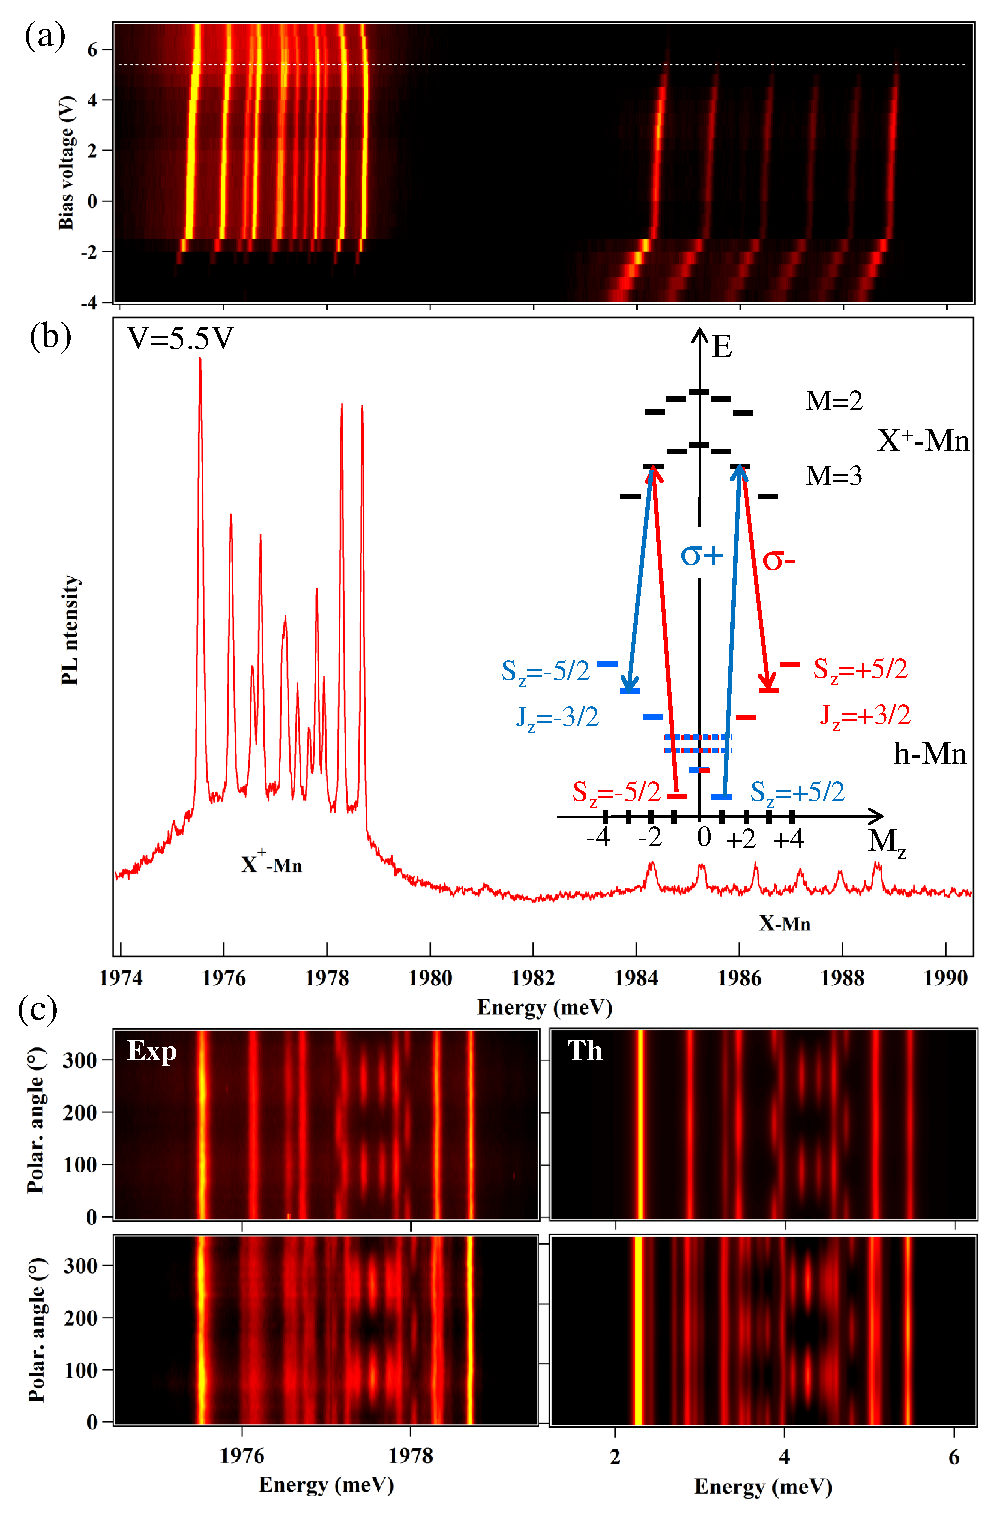
\includegraphics[width=3.1in]{Fig1.eps}
\caption{(a) Color scale plot of the PL intensity of the studied Mn doped QD inserted in Schottky structure showing the emission of the neutral ($X-Mn$) and positively charged ($X^+-Mn$) exciton as a function of energy and bias voltage. (b) PL of the Mn-doped QD under a positive bias voltage of V=5.5V. Inset: Scheme of the energy levels of the ground ($h-Mn$) and excited states ($X^+-Mn$) in a positively charged Mn-doped QD as a function of their angular momentum ($M_z$). (c) Experimental (left) and calculated (right) color-scale plot of the linear polarization dependence of the PL of $X^+-Mn$ at B=0T (top) and B$_\perp$=0.42T (bottom). The parameters used in the calculation are listed in table \ref{paraQD}.}
\label{Fig1}
\end{figure}

A Mn atom in a strained self-assembled CdTe QD exhibits a fine structure dominated by a weak magnetic anisotropy with an easy axis along the QD axis \cite{LeGall2010,LeGall2009,Goryca2014}. Neglecting the small tetrahedral crystal field of the CdTe matrix \cite{Qazzaz1995,Causa1980}, this fine structure is described by the effective spin Hamiltonian

\begin{eqnarray}
\label{cf}
{\cal H}_{Mn,CF}=D_0S^2_z+E(S_y^2-S_x^2)
\end{eqnarray}

\noindent Here, $D_0$ depicts the effect of the biaxial strain and $E$ describes the anisotropy of the strain in the plane of the QD. $D_0$ varies from 0 $\mu$eV (strain free QD \cite{Besombes2014}) to 12 $\mu$eV (strained CdTe layer matched on a ZnTe substrate \cite{LeGall2009}) and typical values around 7 $\mu$eV are usually observed in CdTe QDs \cite{Jamet2013,Goryca2014}.

When a hole is trapped in a QD containing a single Mn, the spin structure is controlled by the hole-Mn exchange interaction

\begin{eqnarray}
\label{state}
{\cal H}_{hMn}^{ex}=I_{hMn}\vec{S}\cdot\vec{J}
\end{eqnarray}

\noindent where I$_{hMn}$ is the exchange energy between the hole and the Mn ($S=5/2$) and $\vec{J}$ is the hole spin operator. In the presence of heavy-hole/light-hole mixing, $\vec{J}$, represented in the basis of the two low energy heavy-hole states, is related to the Pauli matrices by $J_z=3/2\tau_z$ and $J_{\pm}= \xi \tau_{\pm}$ with $\xi=-2\sqrt{3}e^{-2i\theta}\rho_s/\Delta_{lh}$. $\rho_s$ is the coupling energy between heavy and light holes split by the energy $\Delta_{lh}$ and $\theta$ is the angle relative to the [110] axis of the principal axis of the anisotropy (shape and/or strain) responsible for the heavy-hole/light-hole mixing \cite{Fernandez2006,Leger2007}. For a weak valence band mixing, the hole-Mn complex forms a spin ladder with a quantization axis along the QDs growth direction. These states are labelled $|S_z,J_z\rangle$.

The PL of a positively charged Mn-doped QD is presented in figure~\ref{Fig1}(b). When an exciton is injected in the QD loaded with a hole, one has to consider the X$^+$-Mn complex. The structure of X$^+$-Mn with two spin paired holes is dominated by the electron-Mn exchange interaction

\begin{eqnarray}
\label{state}
{\cal H}_{eMn}^{ex}=I_{eMn}\vec{S}\cdot\vec{\sigma}
\end{eqnarray}

\noindent with $\vec{\sigma}$ the electron spin and $I_{eMn}$ the exchange energy between the electron and the Mn. The twelve e-Mn states are split into a ground state sextuplet (total spin M=3) and a fivefold degenerated manifold (total spin M=2) (see inset of Fig.~\ref{Fig1}(b)). These energy levels are labelled $|M,M_z\rangle$.

\begin{table}[t] \centering
\caption{Values of the parameters used in the model of the positively charged Mn-doped QD presented in figure 1. I$_{eMn}$, I$_{hMn}$, $\frac{\rho_s}{\Delta_{lh}}$, $\theta$, $\eta$ and $T_{eff}$ are used to model the linear polarization intensity map of Fig.~\ref{Fig1}. The other parameters cannot be extracted from the PL measurements and values for typical Mn-doped QDs are chosen for the calculation of the spin dynamics presented in section VI.}
\renewcommand{\arraystretch}{1.0}

\begin{tabular}{lcr}
\hline\hline
Exchange interaction & I$_{eMn}$ &  -175$\mu eV$  \\
& I$_{hMn}$&  345$\mu eV$  \\
Valence band mixing & $\frac{\rho_s}{\Delta_{lh}}$ &  0.09  \\
& $\theta$ &  0 $^{\circ}$  \\
Hole perturbation & $\eta$ &  30$\mu eV$   \\
Effective temperature & $T_{eff}$ &  20 K \\
\hline
g factors  & $g_{e}$ &  -0.4  \\
& $g_{h}$ &  -0.6  \\
& $g_{Mn}$  &  2 \\
Mn fine structure & $D_0$  &  7 $\mu eV$ \\
& $E$  &  1.5 $\mu eV$  \\
\hline\hline
\end{tabular}

%\begin{tabular}{p{0.8cm}p{0.8cm}p{0.8cm}p{0.3cm}p{0.6cm}p{0.6cm}|p{0.6cm}p{0.6cm}p{0.6cm}p{0.6cm}p{0.6cm}}
%\hline\hline
%I$_{eMn}$ & I$_{hMn}$ & $\frac{\rho_s}{\Delta_{lh}}$ & $\theta$    & $\eta$   & $T_{eff}$  & $g_{e}$ & $g_{h}$   & $g_{Mn}$ & $D_0$    &  $E$      \\
%$\mu eV$  & $\mu eV$  &                              & $^{\circ}$  & $\mu eV$ &    K       &         &           &          & $\mu eV$ &  $\mu eV$ \\
%\hline
%  -175    &     345   &        0.09                  &    0        &     30   &   20       &  -0,4   &  0.6      &     2    &    7     &   1.5     \\
%\hline\hline
%\end{tabular}

\label{paraQD}
\end{table}


The exchange coupling between the holes and the Mn introduce a perturbation of their wave function \cite{Besombes2005,Trojnar2013,Besombes2014}, that can be represented for one hole by an effective spin Hamiltonian ${\cal H}_{scat}=-\eta S_z^2$ with $\eta>$0. This perturbation has to be taken into account twice for X$^+$-Mn where two holes interact with the Mn. This perturbation affects the energy of the optical recombination to the hole-Mn ground state and can be observed in the emission spectra \cite{Besombes2014}.

Values of $I_{hMn}$, $I_{eMn}$, $\rho_s/\Delta_{lh}$ and $\eta$ for a given QD can be obtained by comparing the linear polarization dependence of the experimental PL data to the optical transition probabilities calculated with the effective spin model (Fig.~\ref{Fig1}(c)) \cite{Varghese2014}. These parameters are listed in table \ref{paraQD} for the QD presented in figure \ref{Fig1}.


% Plot the calculated energy levels of h-Mn? Influence of the E term on the h-Mn ground states? and describe more in detail



\section{Dynamics of the resonant fluorescence of X$^+$-Mn.}

When scanning a resonant laser on the high energy side of X$^+$-Mn, three main absorptions are observed \cite{Lafuente2015}. These absorptions resonances are labelled (1), (2) and (3) in Fig.~\ref{Fig2}(a). They give rise to a large resonant PL which is cross circularly polarized with the excitation, except for an excitation on (1) which produces unpolarized PL. The corresponding energy levels involved in these absorption are identified in Fig.~\ref{Fig2}(b). They correspond, for a $\sigma+$ laser, to the successive resonant excitation of the electron-Mn levels $|3,+1\rangle$, $|3,+2\rangle$ and $|2,+2\rangle$ \cite{Lafuente2015}. These states can be expressed as linear combinations of the Mn and electron spins $|S_z;\sigma_z\rangle$ coupled by a flip-flop:

\begin{eqnarray}
\label{state}
|3,+1\rangle&=& \frac{1}{\sqrt{6}}(\sqrt{4}|+1/2,\uparrow_e\rangle+\sqrt{2}|+3/2,\downarrow_e\rangle)\\
|3,+2\rangle&=& \frac{1}{\sqrt{6}}(\sqrt{5}|+3/2,\uparrow_e\rangle+\sqrt{1}|+5/2,\downarrow_e\rangle)\\
|2,+2\rangle&=& \frac{1}{\sqrt{6}}(\sqrt{1}|+3/2,\uparrow_e\rangle-\sqrt{5}|+5/2,\downarrow_e\rangle)
\end{eqnarray}

Each of these electron-Mn states is connected with circularly polarized optical transitions to two hole-Mn states in the ground state of the QD. For instance $|3,+2\rangle$ is connected to $|+\frac{3}{2};\Uparrow_h\rangle$ with $\sigma-$ photons and to $|+\frac{5}{2};\Downarrow_h\rangle$ with $\sigma+$ photons. This level structure forms an optical $\Lambda$ system. Under resonant excitation of one high energy level of X$^+$-Mn, only one cross-circularly polarized emission line is observed. It corresponds to the optically allowed recombination on the second branch of the $\Lambda$ system. This recombination occurs with a flip-flop of the electron and Mn spins \cite{Varghese2014,Lafuente2015}. The energy splitting between the resonant absorption and the emission is determined by the splitting of the two ground states of the $\Lambda$ system. It is given by 4$\times$3/2$I_{hMn}\approx2.1 meV$ for an excitation of $|3,+2\rangle$ or $|2,+2\rangle$ and 2$\times$3/2$I_{hMn}\approx1.05 meV$ for an excitation of $|3,+1\rangle$. The weak co-polarized signal, which depends on the excitation intensity, comes from a possible direct weak excitation of the low energy branch of the $\Lambda$ system through the acoustic phonon side-band \cite{Besombes2001}.

\begin{figure}[hbt]
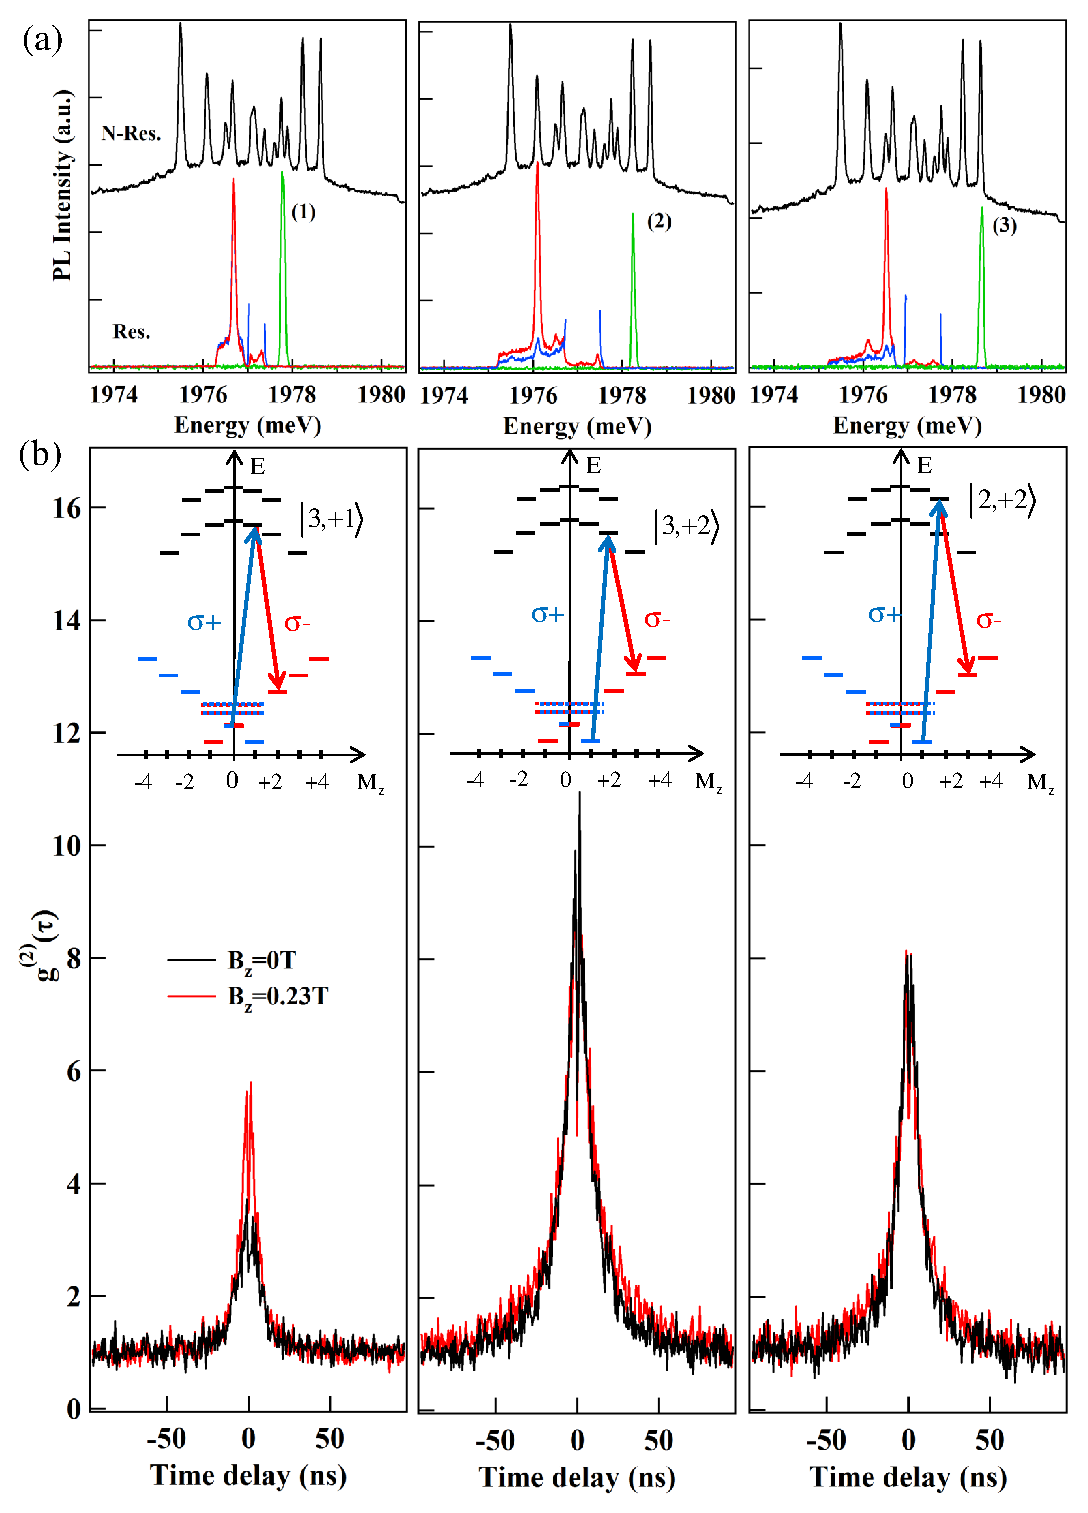
\includegraphics[width=3.3in]{Fig2.eps}
\caption{(a) Non resonant (N-Res.) and resonant (Res.) PL of X$^+$-Mn. Co (blue) and cross (red) circularly polarized PL spectra are collected for three different energies of the CW resonant laser (green). (b) Auto-correlation of the resonant PL for a cross circularly polarized excitation and detection of the e-Mn states $|3,+1\rangle$, $|3,+2\rangle$ and $|2,+2\rangle$. Insets: Energy levels of X$^+$-Mn and identification of the three resonances observed in (a) corresponding to the optical $\Lambda$ systems associated with the e-Mn states $|3,+1\rangle$, $|3,+2\rangle$ and $|2,+2\rangle$.}
\label{Fig2}
\end{figure}

Under resonant excitation of one of the branch of a $\Lambda$ system, a fast optical pumping controlled by the generation rate and the radiative lifetime of the excited state is expected: The population should be stored in the level which is not excited and the resonant PL should vanish. For X$^+$-Mn, the large PL intensity observed under resonant excitation of the high energy branch of the $\Lambda$ systems, similar to the PL intensity obtained under non-resonant excitation, suggests a very inefficient optical pumping of the coupled hole and Mn spins and an efficient spin flip mechanism which links the two ground states.

\begin{figure}[hbt]
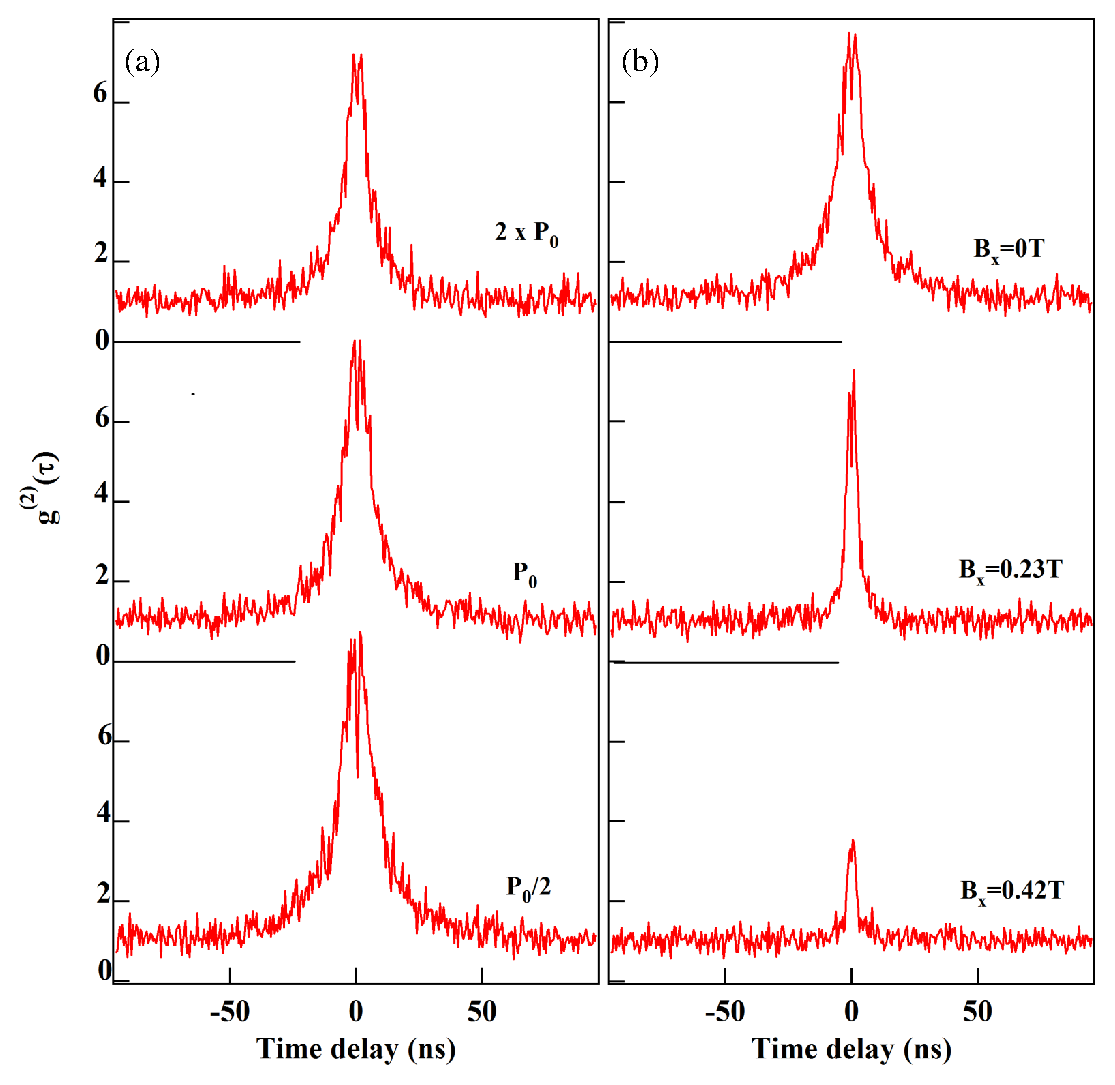
\includegraphics[width=3.1in]{Fig3.eps}
\caption{Excitation power dependence (a) and transverse magnetic field dependence (b) of the auto-correlation of the resonant PL obtained for an excitation on the high energy branch of the $\lambda$ level system associated to the e-Mn state $|2,+2\rangle$.}
\label{Fig3}
\end{figure}

To analyze the dynamics of the coupled carriers and Mn spins under resonant optical excitation, we first use the statistics of the time arrival of the photons given by the second order correlation function $g^{(2)}(\tau)$ of the PL intensity. Fig.\ref{Fig2}(b) shows $g^{(2)}(\tau)$ for the three resonant excitation energies corresponding to the identified optical $\Lambda$ systems. $g^{(2)}(\tau)$ is mainly characterized by a large photon bunching with a full width at half maximum (FWHM) in the 20 ns range. The amplitude of the bunching reaches 9 for line (2) and is slightly weaker for the two other lines. This large bunching reflects an intermittency in the emission of the resonantly excited QD. The bunching signal is not sensitive to a longitudinal magnetic field B$_z$ accept for an excitation on (1) where the bunching amplitude is slightly enhanced under a weak B$_z$.

The presence of a photon bunching is at first sight surprising: under resonant excitation of an isolated $\Lambda$ system, an anti-bunching controlled by the transfer time between the two ground states is indeed expected. A transfer time in the nanosecond range is indeed required to obtain the narrow anti-bunching signal observed near zero delay in the autocorrelation signal (see for instance the auto-correlation at low excitation power in figure~\ref{Fig3}(a)).

In the presence of such fast transfer process connecting the two hole-Mn ground states, a photon bunching in the resonant PL can be explained by a leak outside of the $\Lambda$ level system which is resonantly excited. Under $cw$ resonant excitation, the population is recycled inside the $\Lambda$ system until a spin flip occurs. The resonant PL is then switched off until multiple spin-flips drives back the carriers and Mn spin inside the resonantly driven $\Lambda$ system. With such blinking induced by fluctuations of the carriers and Mn spins, the selected QD line can be either in a ON or OFF state and the amplitude of the bunching is given by the $\Gamma_{Out}/\Gamma_{In}$ the ratio of the transition rates from OFF to ON ($\Gamma_{In}$) and from ON to OFF ($\Gamma_{Out}$). An amplitude of bunching larger than 1 is then expected for the multilevel system considered here where, after a spin relaxation, multiple spin flips are in average required to come back to the initial state ($\Gamma_{In}<\Gamma_{Out}$). The width of the bunching is a measurement of the escape time out of the considered $\Lambda$ level system.

A weak transverse magnetic field significantly reduces the width of the bunching signal (Fig.\ref{Fig3}(b)). As the spin of the hole-Mn complex is highly anisotropic with a large splitting induced by their exchange interaction $S_z.J_z$, the weak transverse magnetic field used in this experiment mainly affects the electron-Mn dynamics. A weak transverse magnetic field couples the different electron-Mn states and induces a leak outside the resonantly excited $\Lambda$ system. Both spin-flips within the hole-Mn or electron-Mn systems can contribute to the bunching signal, but the effect of the weak transverse field shows that the probability of presence in the excited state of the $\Lambda$ system is large. This is consistent with the large excitation intensity used for these auto-correlation measurements which require a high photon count rate.

A slight reduction of the width of the bunching signal is also observed with the increase of the excitation intensity. This shows that the leaks outside a given $\Lambda$ system increases with the probability of presence of the positively charged exciton in the QD.


\section{Resonant optical pumping and spin relaxation of h-Mn}


To analyse how fast the coupled hole-Mn spins can relax back inside the resonantly excited $\Lambda$ system, we performed resonant optical pumping experiments. To first demonstrate the presence of resonant optical pumping and ist efficiency, we excite the high energy branch of the $\Lambda$ systems with trains of resonant light with alternated circular polarization and record the PL of the low energy branch. As observed in Fig.~\ref{Fig4}, for a resonant excitation at the energy of the electron-Mn states $|3,+2\rangle$ or $|2,+2\rangle$, switching the polarization of the excitation from co to cross circular produces a change of the PL intensity with two transients: first, an abrupt PL increase (or decrease), reflecting the population change of the observed spin-polarized charged excitons; then a slower transient with a characteristic time of a few tens of nanoseconds, depending on the laser excitation intensity.

\begin{figure}[hbt]
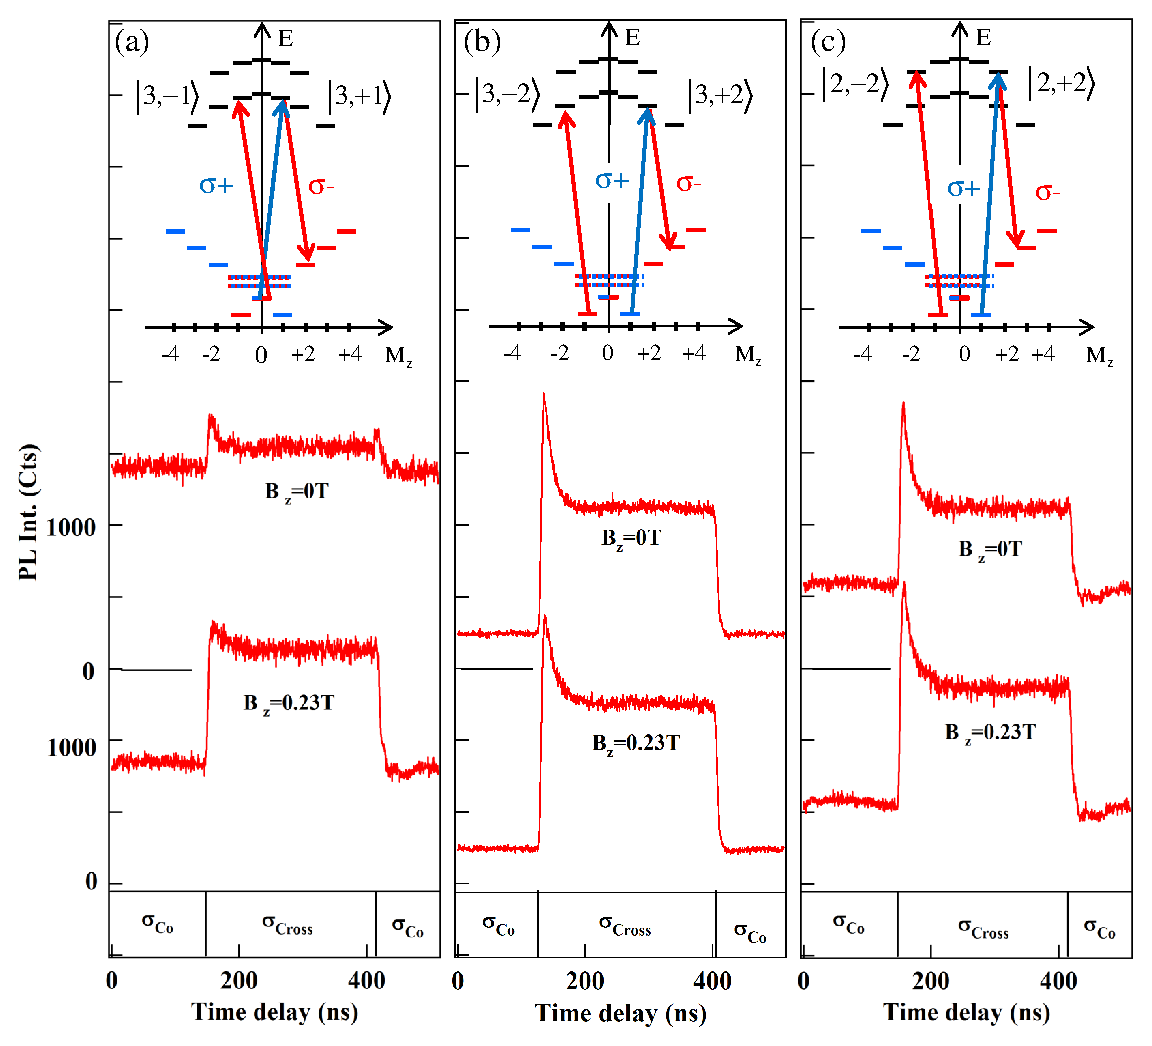
\includegraphics[width=3.4in]{Fig4.eps}
\caption{Resonant optical pumping transients obtained under circular polarization switching of the resonant excitation for the $\Lambda$ systems identified in figure \ref{Fig2} at zero field and under a weak longitudinal magnetic field B$_z$=0.23T. The insets present the corresponding states which are resonantly excited and detected in $\sigma-$ polarization.}
\label{Fig4}
\end{figure}

The progressive decrease of the resonant PL intensity is the signature of an optical pumping of the resonantly excited hole-Mn spin state: the hole-Mn state which is excited is partially emptied when the population is ejected out of the resonantly excited $\Lambda$ system. As presented in figure~\ref{Fig4}, this pumping signal is not sensitive to a longitudinal magnetic field B$_z$ except for an excitation of $|3,+1\rangle$ where a significant intensity difference between co and cross circular polarization is only observed under a weak B$_z$ .

The speed of the optical pumping increases with the excitation intensity. This is presented in the case of a resonant excitation of $|3,+2\rangle$ (or $|3,-2\rangle$) in Fig.~\ref{Fig5}(a). At high excitation intensity, the pumping time saturates to a value similar to the characteristic time of the bunching signal observed in the auto-correlation measurements.

\begin{figure}[hbt]
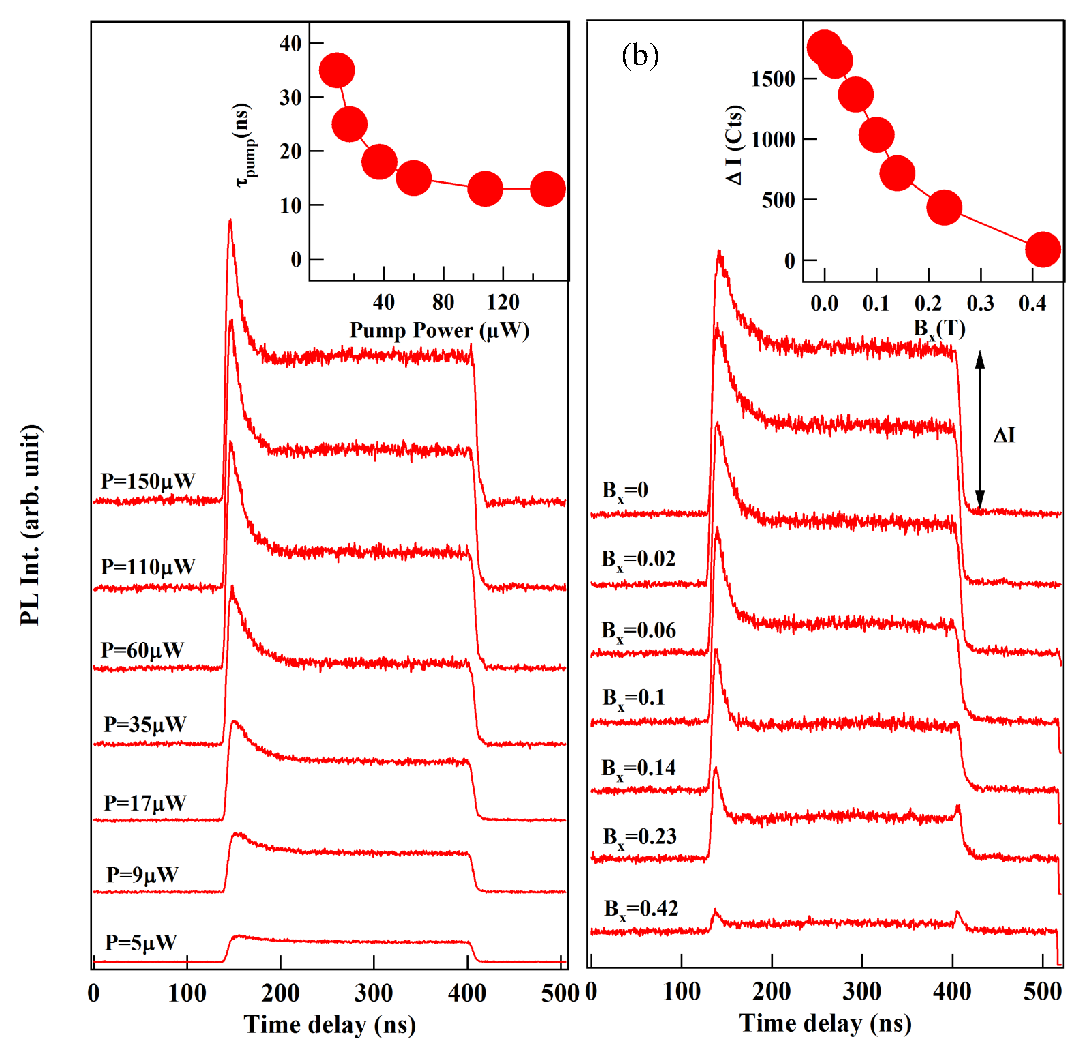
\includegraphics[width=3.3in]{Fig5.eps}
\caption{Excitation power dependence (a) and transverse magnetic field dependence (b) of the optical pumping signal obtained for a resonant excitation on $|3,+2\rangle$. Insets: excitation power dependence of the pumping time and transverse magnetic field dependence of the difference of resonant PL intensity between a $\sigma_{cross}$ and a $\sigma_{co}$ excitation.}
\label{Fig5}
\end{figure}

The pumping signal is also strongly sensitive to a transverse magnetic field. As presented in Fig.~\ref{Fig5}(b), under a weak transverse field, we first observe an increase of the speed of the pumping together with a decrease of the amplitude of the signal when the transient time reaches the time resolution of the set-up (around 10 ns). For a large transverse field (B$_\perp$=0.42T), the co and cross circularly polarized resonant PL intensities are identical (see the inset of Fig.~\ref{Fig5}(b)) and similar pumping transients are observed when switching from co to cross or from cross to co circular polarization.

\begin{figure}[hbt]
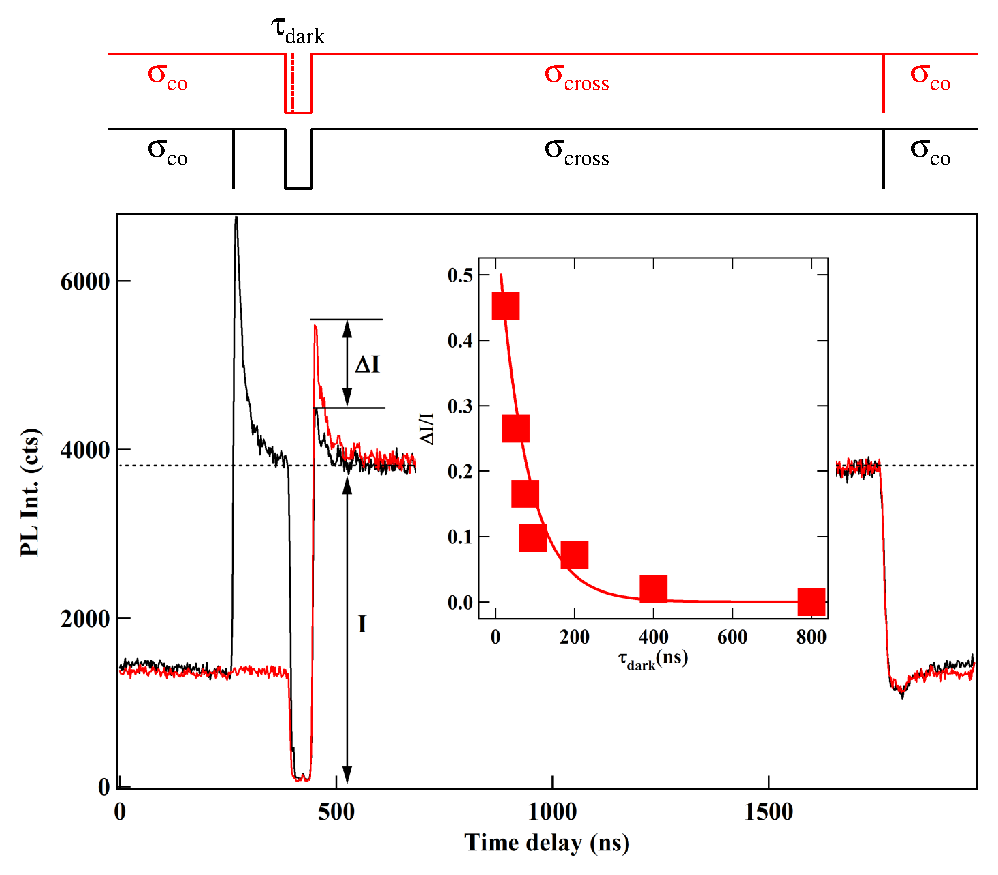
\includegraphics[width=3.3in]{Fig6.eps}
\caption{Optical pumping experiment for an excitation of $|3,+2\rangle$ with modulated circular polarization. A dark time ($\tau_{dark} = 50ns$) is introduced either before (black) or during (red) the change of circular polarization. The black and red diagrams present the corresponding resonant excitation sequences. The inset presents the variation of the ratio $\Delta I/I$ as a function of $\tau_{dark}$. The solid line is an exponential fit with $\tau_{relax} = 80 ns$.}
\label{Fig6}
\end{figure}

To observe the relaxation of the prepared non–equilibrium distribution of the hole-Mn spins, the circularly polarized pump laser is switched off during a dark time $\tau_{dark}$.  The amplitude of the pumping transient after $\tau_{dark}$ depends on the hole-Mn spin relaxation. A dark time of 50 ns is enough to observe the reappearance of a significant pumping transient (Fig.~\ref{Fig6}). For comparison and for a better sensitivity of the measurement, the pumping transient observed in the absence of initial preparation of the hole-Mn spin (i.e. when switching of the circular polarization during the dark time) is also presented (red trace in Fig.~\ref{Fig6}). The normalized difference of the amplitude of these two transients, $\Delta I/I$, as a function of $\tau_{dark}$ is presented in the inset of Fig.\ref{Fig6}. This measurement shows that, when the optical excitation is off, it takes around 80 ns to the hole-Mn spin to come back to the ground state of the excited $\Lambda$ system.

If the optical pumping was storing the hole-Mn spin in the branch of the $\Lambda$ system which is not optically excited, its characteristic time would be controlled by the exciton radiative lifetime and the generation rate. With a relaxation time in the 100 ns range, as observed experimentally, the pumping should take place within a few nanoseconds. Another source of spin pumping can be the leak outside the resonantly excited $\lambda$ system. In this case, the speed of the pumping is controlled by the leakage time and, as observed experimentally, the pumping time is similar to the width of the photon bunching signal. This mechanism of pumping is confirmed by the observed  transverse magnetic field dependence. The acceleration of the optical pumping in transverse magnetic field (Fig.~\ref{Fig5}(b)) has the same origin as the decrease of the width of the bunching signal. By mixing the different electron-Mn states, the transverse field enhance the leakage probability out of the resonantly driven $\Lambda$ system and decreases the corresponding optical pumping time.


\section{Model of coupled hole and Mn spin dynamics}

The observed resonant PL amplitude of X$^+$-Mn and its dynamics can be qualitatively explained if a fast (nanosecond) and efficient spin transfer mechanism connects the two hole-Mn ground states of the $\Lambda$ systems.

In the presence of valence band mixing, the two ground states of a given $\Lambda$ system are coherently coupled by a hole-Mn flip-flop induced by the exchange interaction ${\cal H}_{hMn}^{ex}$. However, as the splitting between these states ($\Delta=4\times3/2I_{hMn}$ for the $\Lambda$ system associated with $|3,+2\rangle$ for instance) is large compared with the coupling term ($W=\sqrt{15}\frac{\rho}{\Delta_{lh}}I_{hMn}$ for the $\Lambda$ system associated with $|3,+2\rangle$), the coherent transfer between the two states is weak. With a large valence band mixing $\frac{\rho}{\Delta_{lh}}=0.1$ as observed in the dot discussed in this paper, this leads for the $\Lambda$ system associated with $|3,+2\rangle$ to a fast oscillation of the population between the two hole-Mn ground states with a maximum amplitude of about 1.6\% and an average population transfer efficiency of 0.8\% \cite{Cohen}.

With only this coherent process for the population transfer, after a resonant excitation and an optical recombination of the charged exciton on the low energy branch of the $\Lambda$ system, the QD would be off more than 99\% of the time. This is not compatible with the large PL intensity obtained under resonant $cw$ excitation. The resonant excitation should also lead to a fast optical pumping in the nanosecond range, controlled by the radiative lifetime and generation rate of exciton. In addition, the system being most of the time in the ground state (more than 99\% of the time), the dynamics of the resonantly driven $\Lambda$ system, probed in the auto-correlation or optical pumping signal should be insensitive to a weak transverse magnetic field. To explain the observed large amplitude and the dynamics of the resonant PL of X$^+$-Mn, one has to find a more efficient transfer mechanism between the two hole-Mn ground states of the $\Lambda$ systems.

We propose an intrinsic mechanism for the hole-Mn flip-flop at low temperature resulting from a deformation induced exchange interaction \cite{Tsitsishvili2003,Roszak2007}. We show here that hole-Mn states are coupled via the interplay of the exchange interaction and the lattice deformation induced lh-hh mixing. We will consider here the two hole-Mn states $|+\frac{3}{2};\Uparrow_h\rangle$ and $|+\frac{5}{2};\Downarrow_h\rangle$ in the ground states of the $\Lambda$ system associated with the electron-Mn levels $|3,+2\rangle$ and $|2,+2\rangle$. Similar results could be obtained with the other $\Lambda$ systems.

First, let us notice that the hole-Mn exchange interaction couples the heavy-hole ($\Uparrow_h,\Downarrow_h)$ and light-hole $(\uparrow_h,\downarrow_h)$ levels split by $\Delta_{lh}$. To the first order in $I_{hMn}/\Delta_{lh}$, the two ground states of the $\Lambda$ system considered here $|+\frac{3}{2};\Uparrow_h\rangle$ and $|+\frac{5}{2};\Downarrow_h\rangle$ can be written:

\begin{eqnarray}
\label{state}
\widetilde{|+\frac{5}{2};\Downarrow_h\rangle}=|+\frac{5}{2};\Downarrow_h\rangle-\frac{\sqrt{15}}{2}\frac{I_{hMn}}{\Delta_{lh}}|+\frac{3}{2};\downarrow_h\rangle\nonumber\\
\widetilde{|+\frac{3}{2};\Uparrow_h\rangle}=|+\frac{3}{2};\Uparrow_h\rangle-\frac{\sqrt{15}}{2}\frac{I_{hMn}}{\Delta_{lh}}|+\frac{5}{2};\uparrow_h\rangle
\end{eqnarray}

\noindent where we neglect the exchange energy shifts of the hole levels much smaller than $\Delta_{lh}$.


Phonon-induced deformations comes into play via the off diagonal terms of the Bir-Pikus Hamiltonian:

\begin{eqnarray}
\label{HBP}
H_{BP}=a\sum_i\epsilon_{ii}+b\sum_i\epsilon_{ii}\left(J_i^2-\frac{1}{3}J^2\right)\nonumber\\
+\frac{2d}{\sqrt{3}}\sum_{i>j}\{J_i,J_j\}\epsilon_{ij}
\end{eqnarray}

\noindent where $\epsilon_{ij}$ are the strain tensor components with $\epsilon_{ij}$=$\epsilon_{ji}$ and $\{J_i,J_j\}=1/2(J_iJ_j+J_jJ_i)$. Phonon vibrations couple the perturbed hole-Mn states $\widetilde{|+5/2\Downarrow_h\rangle}$ and $\widetilde{|+3/2\Uparrow_h\rangle}$ through the Hamiltonian term

\begin{eqnarray}
\label{int}
\widetilde{\langle+\frac{5}{2};\Downarrow_h|}H_{BP}\widetilde{|+\frac{3}{2};\Uparrow_h\rangle}=-\sqrt{15}\frac{I_{hMn}}{\Delta_{lh}}P^*
\end{eqnarray}

\noindent with

\begin{eqnarray}
\label{P}
P=\left(\frac{\sqrt{3}}{2}b(\epsilon_{xx}-\epsilon_{yy})-id\epsilon_{xy}\right)
\end{eqnarray}

\noindent a deformation dependent non-diagonal term of $H_{BP}$ \cite{Tsitsishvili2003,Roszak2007}. This coupling is a result of an interplay between the hole-Mn exchange interaction and the deformation: neither the exchange interaction nor the deformation perturbation alone can couple these states.

According to (\ref{int}), an effective Hamiltonian describing the discussed interaction mechanism with phonons in the subspace $\{|+\frac{5}{2};\Uparrow_h\rangle,|+\frac{5}{2};\Downarrow_h\rangle, |+\frac{3}{2};\Uparrow_h\rangle,|+\frac{3}{2};\Downarrow_h\rangle\}$  is

\begin{eqnarray}
\label{Hint}
H_{int}=-\sqrt{15}\frac{I_{hMn}}{\Delta_{lh}}P^*|+\frac{5}{2};\Downarrow_h\rangle\langle+\frac{3}{2};\Uparrow_h|+H.c
\end{eqnarray}

The spin decay rates from $|+\frac{3}{2};\Uparrow_h\rangle$ to $|+\frac{5}{2};\Downarrow_h\rangle$ accompanied by emission of phonons is given by Fermi's golden rule

\begin{eqnarray}
\label{fermi}
\tau^{-1}&=&\frac{2\pi}{\hbar}\sum_{k}\left|\langle+\frac{5}{2};\Downarrow_h;\psi;n_k+1|H_{int}|+\frac{3}{2};\Uparrow_h;\psi;n_k\rangle\right|^2\nonumber\\
&\times&\delta(\hbar\omega_0-\hbar\omega_{k})
\end{eqnarray}

\noindent where $\hbar\omega_0$ is the energy splitting between $|+\frac{5}{2};\Downarrow_h\rangle$ and $|+\frac{3}{2};\Uparrow_h\rangle$, $n_k$ the number of phonons in mode $k$ and $\psi$ the orbital part of the hole wave function.

To evaluate the matrix element in (\ref{fermi}) we use the strain tensor components $\epsilon_{ij}$ given by

\begin{eqnarray}
\label{eps}
{
\epsilon_{ij}=\frac{1}{2}\left(\frac{\partial u_i}{\partial r_j}+\frac{\partial u_j}{\partial r_i}\right)
}
\end{eqnarray}

\noindent where $\overrightarrow{u}(\overrightarrow{r})$ is the local displacement field. The quantized displacement field can be written in the real space \cite{Mahan}:

\begin{eqnarray}
\label{u}
{
\overrightarrow{u}(\overrightarrow{r})=i\sum_{k,\lambda}\sqrt{\frac{\hbar}{2\rho N \nu_0 \omega_{k,\lambda}}}\overrightarrow{e}_{k,\lambda}(b^\dag_{k,\lambda}+b_{-k,\lambda})e^{i\overrightarrow{k}\overrightarrow{r}}
}
\end{eqnarray}

\noindent where N is the number of unit cells in the crystal, $\nu_0$ is the volume of a cell and $\rho$ the mass density. $b^\dag_{k,\lambda}$ ($b_{k,\lambda}$) is the creation (annihilation) operator of phonon in the mode $(k,\lambda)$ of energy $\hbar\omega_{k\lambda}$ and unit polarization vector $\overrightarrow{e}_{k,\lambda}$. In zinc-blend crystals there are two transverse acoustic phonon branches $\lambda=t_1, t_2$ and one longitudinal acoustic phonon branch $\lambda=l$. The polarization vectors of these phonons branches are given by \cite{Woods2004}

\begin{eqnarray}
\overrightarrow{e}_{k,l}&=&\frac{\overrightarrow{k}}{k}=\frac{1}{k}(k_x,k_y,k_z)\nonumber\\
\overrightarrow{e}_{k,t_1}&=&\frac{1}{kk_{\bot}}(k_xk_z,k_yk_z,-k_{\bot}^2)\nonumber\\
\overrightarrow{e}_{k,t_2}&=&\frac{1}{k_{\bot}}(k_y,-k_x,0)
\end{eqnarray}

\noindent with $k_{\bot}=\sqrt{k_x^2+k_y^2}$. Upon substitutions given by (\ref{eps}) and (\ref{u}) we obtain for the matrix element in (\ref{fermi}):


\begin{eqnarray}
&&|M_{k,\lambda}|^2=\left(\frac{I_{hMn}}{\Delta_{lh}}\right)^2\frac{15\hbar}{2\rho N \nu_0\omega_{k,\lambda}}\left(n_B(\omega_{k,\lambda})+1)\right)\nonumber\\
&\times&\left(\frac{3b^2}{4}(k_xe_{x,\lambda}-k_ye_{y,\lambda})^2+\frac{d^2}{4}(k_xe_{y,\lambda}+k_ye_{x,\lambda})^2\right)\nonumber\\
&\times&|\mathcal{F}_{\lambda}(\overrightarrow{k})|^2
\end{eqnarray}

\noindent with

\begin{eqnarray}
\mathcal{F}_{\lambda}(\overrightarrow{k})=\int_{-\infty}^{\infty}d^3r\psi^*(\overrightarrow{r})e^{i\overrightarrow{k}\overrightarrow{r}}\psi^(\overrightarrow{r})
\end{eqnarray}

\noindent and $n_B(\omega_{k,\lambda})=
1/(e^{\hbar\omega_{k,\lambda}/K_BT}-1)$, the thermal phonon distribution function. For a Gaussian hole wave function with in-plane and z-direction parameters l$_{\bot}$ and l$_z$ respectively (full width at half maximum $2\sqrt{2\ln2}l_i$)

\begin{eqnarray}
\psi(\overrightarrow{r})=\frac{1}{\pi^{3/4}l_{\bot}\sqrt{l_z}}e^{-\frac{1}{2}\left(\left(\frac{r_{\bot}}{l_{\bot}}\right)^2+\left(\frac{z}{l_z}\right)\right)}
\end{eqnarray}

\noindent the form factor $\mathcal{F}_{\lambda}(\overrightarrow{k})$ becomes

\begin{eqnarray}
\mathcal{F}_{\lambda}(\overrightarrow{k})=e^{-\frac{1}{4}\left(\left(l_{\bot}k_{\bot}\right)^2+\left(l_zk_z\right)^2\right)}
\end{eqnarray}


\begin{table}[hbt] \centering
\caption{Material (CdTe or ZnTe) \cite{Adachi2005} and QD parameters used in the calculation of the coupled hole and Mn spin relaxation time.}
\begin{tabular}{lcr}
\hline\hline
CdTe& &\\
\hline
Deformation potential constants & b &  -1.0 eV  \\
& d &  -4.4 eV  \\
Longitudinal sound speed & c$_l$ &  3300 m/s  \\
Transverse sound speed & c$_t$ &  1800 m/s  \\
Density & $\rho$ &  5860 kg/m$^3$  \\
\hline
ZnTe& &\\
\hline
Deformation potential constants & b &  -1.4 eV  \\
& d &  -4.4 eV  \\
Longitudinal sound speed & c$_l$ &  3800 m/s  \\
Transverse sound speed & c$_t$ &  2300 m/s  \\
Density & $\rho$ &  5908 kg/m$^3$  \\
\hline
Quantum dot& &\\
\hline
Hole Mn exchange energy & I$_{hMn}$ &  0.35 meV  \\
hh-lh exciton splitting&  $\Delta_{lh}$&  15 meV  \\
Hole wave function widths: & &   \\
- in plane & l$_{\bot}$ &3.0 nm   \\
- z direction  & l$_z$ &1.25 nm   \\
\hline\hline
\end{tabular}
\label{paraph}
\end{table}


Considering a linear dispersion of acoustic phonons $\omega_{k,\lambda}=c_{\lambda}k$ and in spherical coordinates with $\overrightarrow{k}=k(\sin\theta\cos\varphi,\sin\theta\sin\varphi,\cos\theta)$, the explicit formula of the decay rate (\ref{fermi}) is

\begin{eqnarray}
\tau^{-1}&=&\sum_{\lambda}\frac{15}{(2\pi)^2}\left(\frac{I_{hMn}}{\Delta_{lh}}\right)^2\left(\frac{\omega_0}{c_{\lambda}}\right)^3\frac{\pi}{2\hbar\rho c_{\lambda}^2}\left(\frac{3b^2}{4}+\frac{d^2}{4}\right)\nonumber\\
&\times&\left(n_B(\omega_0)+1)\right)\int_0^{\pi}d\theta\sin\theta|\mathcal{F}_{\lambda}(\omega_0,\theta)|^2G_{\lambda}(\theta)
\end{eqnarray}

\noindent where we used the continuum limit ($\sum_k\rightarrow V/(2\pi)^3\int d^3k$) and integrated over $k$ and $\varphi$. The summation is taken over the acoustic phonon branches $\lambda$ of corresponding sound velocity c$_{\lambda}$ and the geometrical form factors $G_{\lambda}(\theta)$ are given by

\begin{eqnarray}
G_{l}(\theta)&=&\sin^4\theta\nonumber\\
G_{t_1}(\theta)&=&\sin^2\theta\cos^2\theta\nonumber\\
G_{t_2}(\theta)&=&\sin^2\theta
\end{eqnarray}

\begin{figure}[hbt]
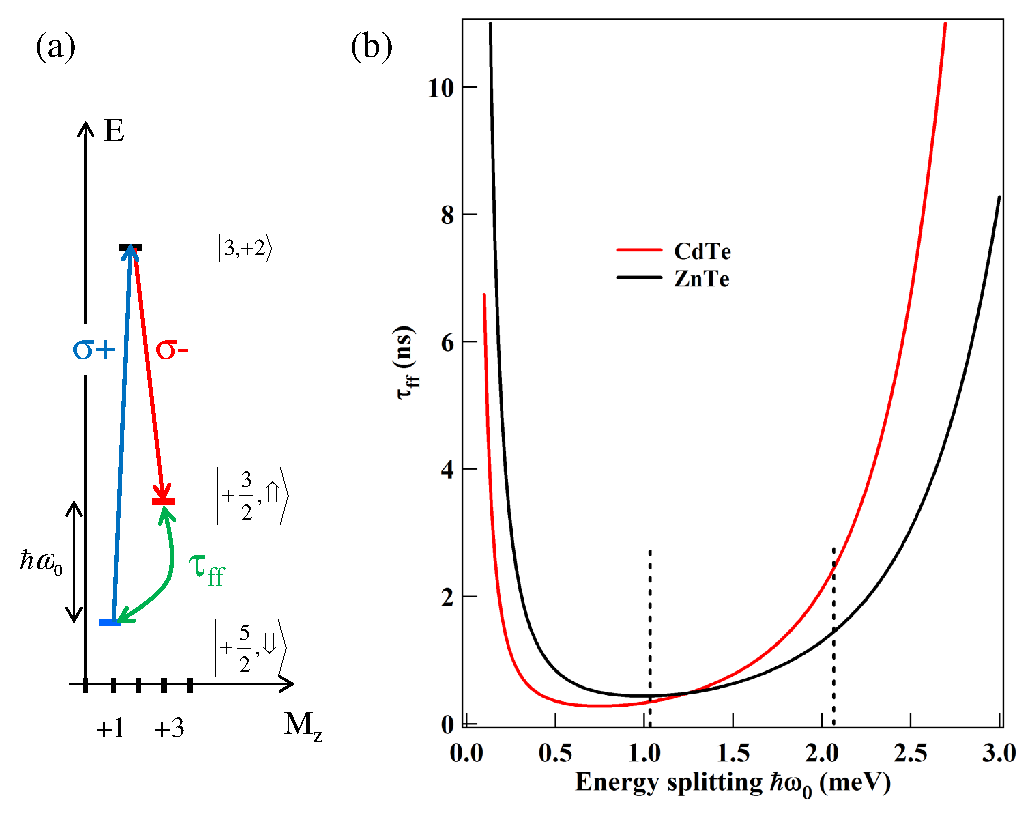
\includegraphics[width=3.3in]{Fig7.eps}
\caption{(a) Scheme of the energy levels of an optical $\Lambda$ system extracted from the full level structure of a positively charged QD (Fig. \ref{Fig1}(b)). (b) Relaxation rates between the two h-Mn ground states of the $\Lambda$ system $\tau_{ff}$ calculated with the material and QD parameters listed in table \ref{paraph} and a temperature T=7K. The vertical lines show the energy splitting of the hole-Mn states involved in the optical $\Lambda$ systems identified in Fig.~\ref{Fig2}.}
\label{Fig7}
\end{figure}


In the numerical calculation of the spin flip rates presented in Fig.\ref{Fig7} we use the material parameters of CdTe or ZnTe and the typical parameters for self-assembled CdTe/ZnTe QDs listed in Table \ref{paraph}. The calculated relaxation time strongly depend on the energy separation between the hole-Mn levels. This energy dependence is controlled by the size of the hole wave-function. The estimated flip-flop time also depends on the phonon induced mixing of the ground heavy-hole states with the higher energy light-hole levels. In our simple model, this mixing is controlled by a parameter $\Delta_{lh}$  which describes more complex effects such coupling with ground state light-holes in the barriers \cite{Michler2003} or effective reduction of heavy-hole/light-hole splitting due to a presence of a dense manifold of heavy-hole like QD states lying between the confined heavy-hole and light-hole levels \cite{Bester2015}. For a hole confined in a self-assembled QD formed by a Cd$_x$Zn$_{1-x}$Te alloy, the flip-flop time $\tau_{ff}$ can be easily bellow 2 ns in the energy separation range of hole-Mn spin levels in typical magnetic QDs (vertical lines in Fig.\ref{Fig7}(b)) with an effective heavy-hole/light-hole splitting $\Delta_{lh}$=15meV.


\section{Model of the carrier-Mn spin dynamics under resonant excitation}


Using the level scheme presented in Fig.\ref{Fig1}(b) for a positively charged Mn-doped QD and the estimated hole-Mn flip-flop rates, we can calculate the time evolution of the 24x24 density matrix $\varrho$ describing the population and the coherence of the 12 electron-Mn states on the excited state and the 12 hole-Mn states on the ground state. In the Markovian approximation, the master equation which governs the evolution of $\varrho$ can be written in a general form (Lindblad form) as:

\begin{equation}
\label{Lindblad} {\frac{\partial\varrho}{\partial t}=\frac{-i}{\hbar}[{\cal H},\varrho]+L\varrho}
\end{equation}

\noindent ${\cal H}$ is the Hamiltonian of the complete system (electron-Mn and hole-Mn):

\begin{eqnarray}
{\cal H}_{e-Mn}=I_{eMn}\vec{S}\cdot\vec{\sigma}-2\eta S_z^2+D_0S^2_z+E(S_y^2-S_x^2)\nonumber\\
+g_{Mn}\mu_B\vec{S}\cdot\vec{B}+g_{e}\mu_B\vec{\sigma}\cdot\vec{B}
\end{eqnarray}

\noindent and

\begin{eqnarray}
{\cal H}_{h-Mn}=I_{hMn}\vec{S}\cdot\vec{J}-\eta S_z^2+D_0S^2_z+E(S_y^2-S_x^2)\nonumber\\
+g_{Mn}\mu_B\vec{S}\cdot\vec{B}+g_{h}\mu_B\vec{J}\cdot\vec{B}
\end{eqnarray}

In (\ref{Lindblad}), $L\varrho$ describes the coupling or decay channels resulting from an
interaction with the environment \cite{Exter2009, Roy2011, Jamet2013}. The population transfers from level $j$ to level $i$ in an irreversible process associated with a coupling to a reservoir is described by $L_{inc,j\rightarrow i}\varrho$:

\begin{eqnarray}
\label{inc}
L_{inc,j\rightarrow i}\varrho=\frac{\Gamma_{j\rightarrow i}}{2}(2|i\rangle\langle j|\varrho|j\rangle\langle i| -\varrho|j\rangle\langle j|-|j\rangle\langle j|\varrho)
\end{eqnarray}

\noindent where $\Gamma_{j\rightarrow i}$ is the incoherent relaxation rate from level $j$ to level $i$. This operator describes the radiative decay of the exciton (irreversible coupling to the photon modes) or the relaxation of the carriers or Mn spin (irreversible coupling to the phonon modes). Such term can also be used to describe the optical generation of an exciton in the low excitation regime where the energy shift induced by the coupling with the laser field is neglected.

A pure dephasing (i.e. not related to an exchange of energy with a reservoir) can also be introduced for the different spins and described by $L_{deph,jj}\varrho$:

\begin{eqnarray}
\label{deph} {L_{deph,jj}\varrho=\frac{\gamma_{jj}}{2}(2|j\rangle\langle j|\varrho|j\rangle\langle j| -\varrho|j\rangle\langle j|-|j\rangle\langle j|\varrho)}
\end{eqnarray}

\noindent where $\gamma_{jj}$ is a pure dephasing rate of level $j$.

To identify the main contribution to the observed spin fluctuations, we first modelled the auto-correlation of the resonant PL using the full spin level structure of a p-doped magnetic QD. For a qualitative description of the observed spin dynamics, we use as an example the Mn-doped QD parameters extracted from the linear polarization intensity map listed in table \ref{paraQD} and reasonable order of magnitude for the spin relaxation times.

To limit the number of parameters and simplify the model we consider that the spin dynamics in the excited state is controlled by $\mathcal{H}_{eMn}^{ex}$, the generation rate of excitons 1/$\tau_g$ and their radiative lifetime $\tau_r$=0.3ns. The coherence of the coupled electron-Mn spins is limited by a pure dephasing term $T_2^{eMn}$=0.5 ns, typical value measured in charged Mn-doped QDs under pulsed resonant excitation \cite{Lafuente2015}.

For the hole-Mn system in the ground state, we take into account a spin relaxation time of the Mn in the exchange field of the hole, $\tau_{Mn}$, describing relaxation channels involving a change of the Mn spin by one unit. This spin relaxation channel is introduced for a general description but its characteristic time (in the $\mu$s range) is however long compared to the time-scale of the dynamics considered in the resonant PL experiments and will not qualitatively affect the calculated time evolution.

Because of the presence of valence band mixing in the QDs, spin flip of the hole independently of the Mn are expected to be more efficient. Spin flip time in the 10 ns range have indeed been calculated for a hole in the exchange field of a Mn spin and are responsible of the optical pumping of the Mn in a neutral QD \cite{Cao2011,Cywinski2010}. Relaxation time of the hole spin around 5 ns has also been measured at zero magnetic field in negatively charged CdTe/ZnTe QDs \cite{LeGall2012}. We then include in the model spin flips of the hole by one unit with a characteristic time $\tau_{h}$=10ns.

The phonon induced hole-Mn flip-flops $\tau_{ff}$ are also introduced between the two hole-Mn ground states of each $\Lambda$ system. For a general qualitative description, an additional pure dephasing time ($T_2^{hMn}$) is also included in the dynamics of the hole-Mn system with a Lindblad term of the form (\ref{deph}). We cannot extract this parameter from the experiments. We take $T_2^{hMn}$= 5 ns, slightly longer than what was measured for electron-Mn, as the hole-Mn system is highly split and less sensitive to effective fluctuating magnetic field such as the one produced by nuclear spins for instance \cite{LeGall2012,Houel2014}.

\begin{figure}[hbt]
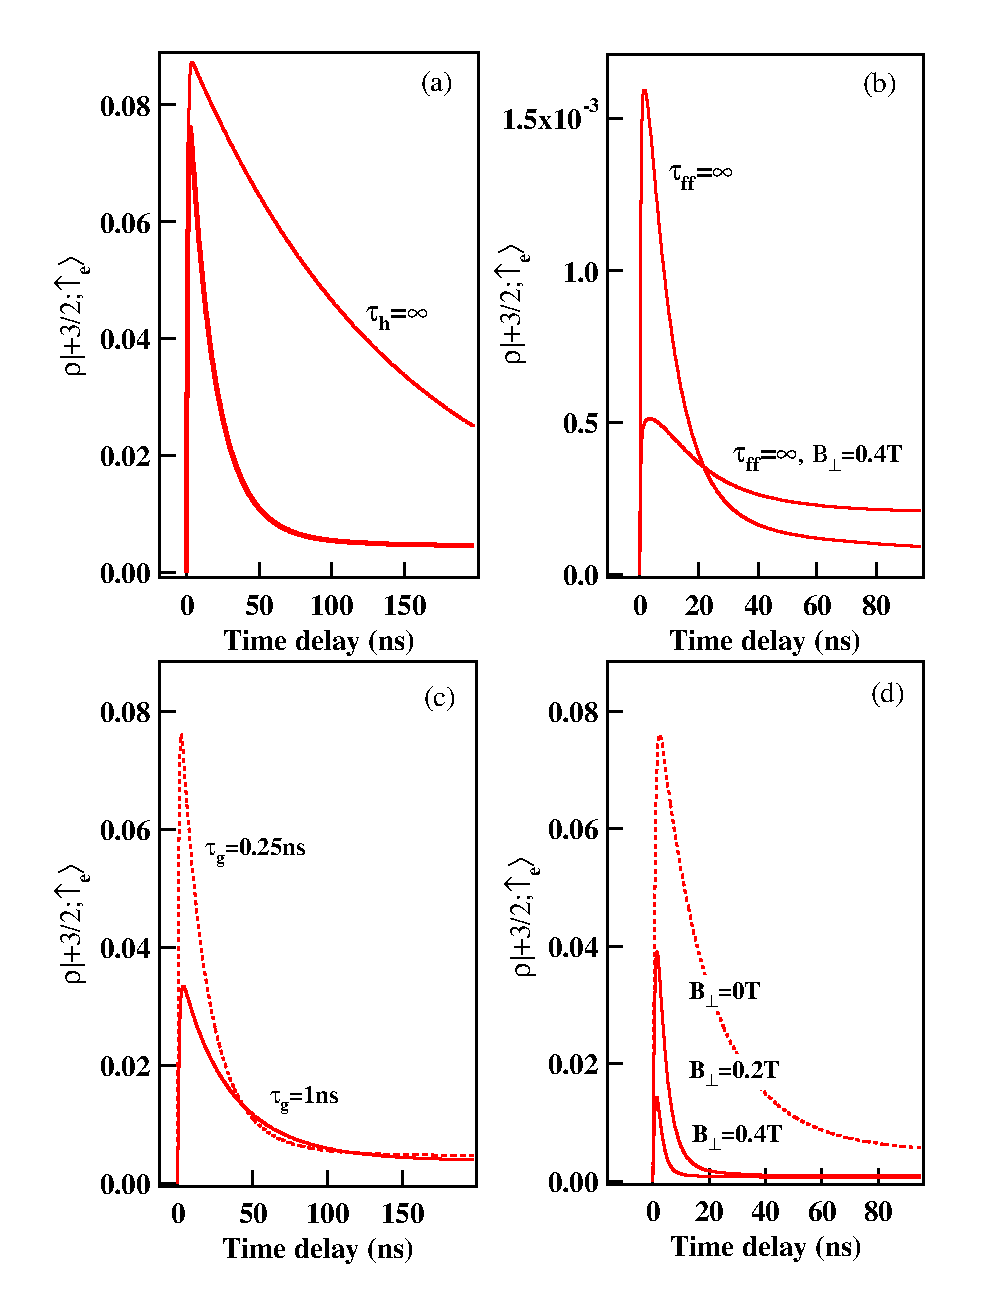
\includegraphics[width=3.3in]{Fig8.eps}
\caption{(a) Calculated time evolution of $\rho_{|+\frac{3}{2},\uparrow_e\rangle}(t)$ with the QD parameters listed in table \ref{paraQD} and (unless specified) $\tau_r$=0.3ns, $\tau_{Mn}$=5 $\mu$s, $\tau_h$=10ns, $\tau_g$=0.25 ns, $\tau_{ff}$=1.5 ns, $T_2^{hMn}$= 5 ns, $T_2^{eMn}$= 0.5 ns, T=10K and B$_{\perp}$=0. (b) (c) and (d) illustrate the influence on $\rho_{|+\frac{3}{2},\uparrow_e\rangle}(t)$ of $\tau_{ff}$, $\tau_g$ and $B_{\perp}$ respectively.}
\label{Fig8}
\end{figure}

The transition rates $\Gamma_{\gamma\rightarrow\gamma'}$ between the different states of h-Mn depend on their energy separation $E_{\gamma\gamma'}=E_{\gamma'}-E_{\gamma}$. Here we use $\Gamma_{\gamma\rightarrow\gamma'}$=1/$\tau_{i}$ if $E_{\gamma\gamma'}<0$ and $\Gamma_{\gamma\rightarrow\gamma'}$=1/$\tau_{i}e^{-E_{\gamma\gamma'}/k_BT}$ if $E_{\gamma\gamma'}>0$ \cite{Govorov2005,Cao2011}. This accounts for a thermalization among the 12 hole-Mn levels with an effective spin temperature $T$. The optical excitation ($\tau_g=1/\Gamma_g$), the exciton recombination ($\tau_r$), the Mn spin relaxation ($\tau_{Mn}$), the hole spin relaxation ($\tau_{h}$) and the phonon induced transfer time $\tau_{ff}$ produce an irreversible population transfer from level $\gamma$ to level $\gamma'$ and are described by Lindblad terms (\ref{inc}).

\begin{figure}[hbt]
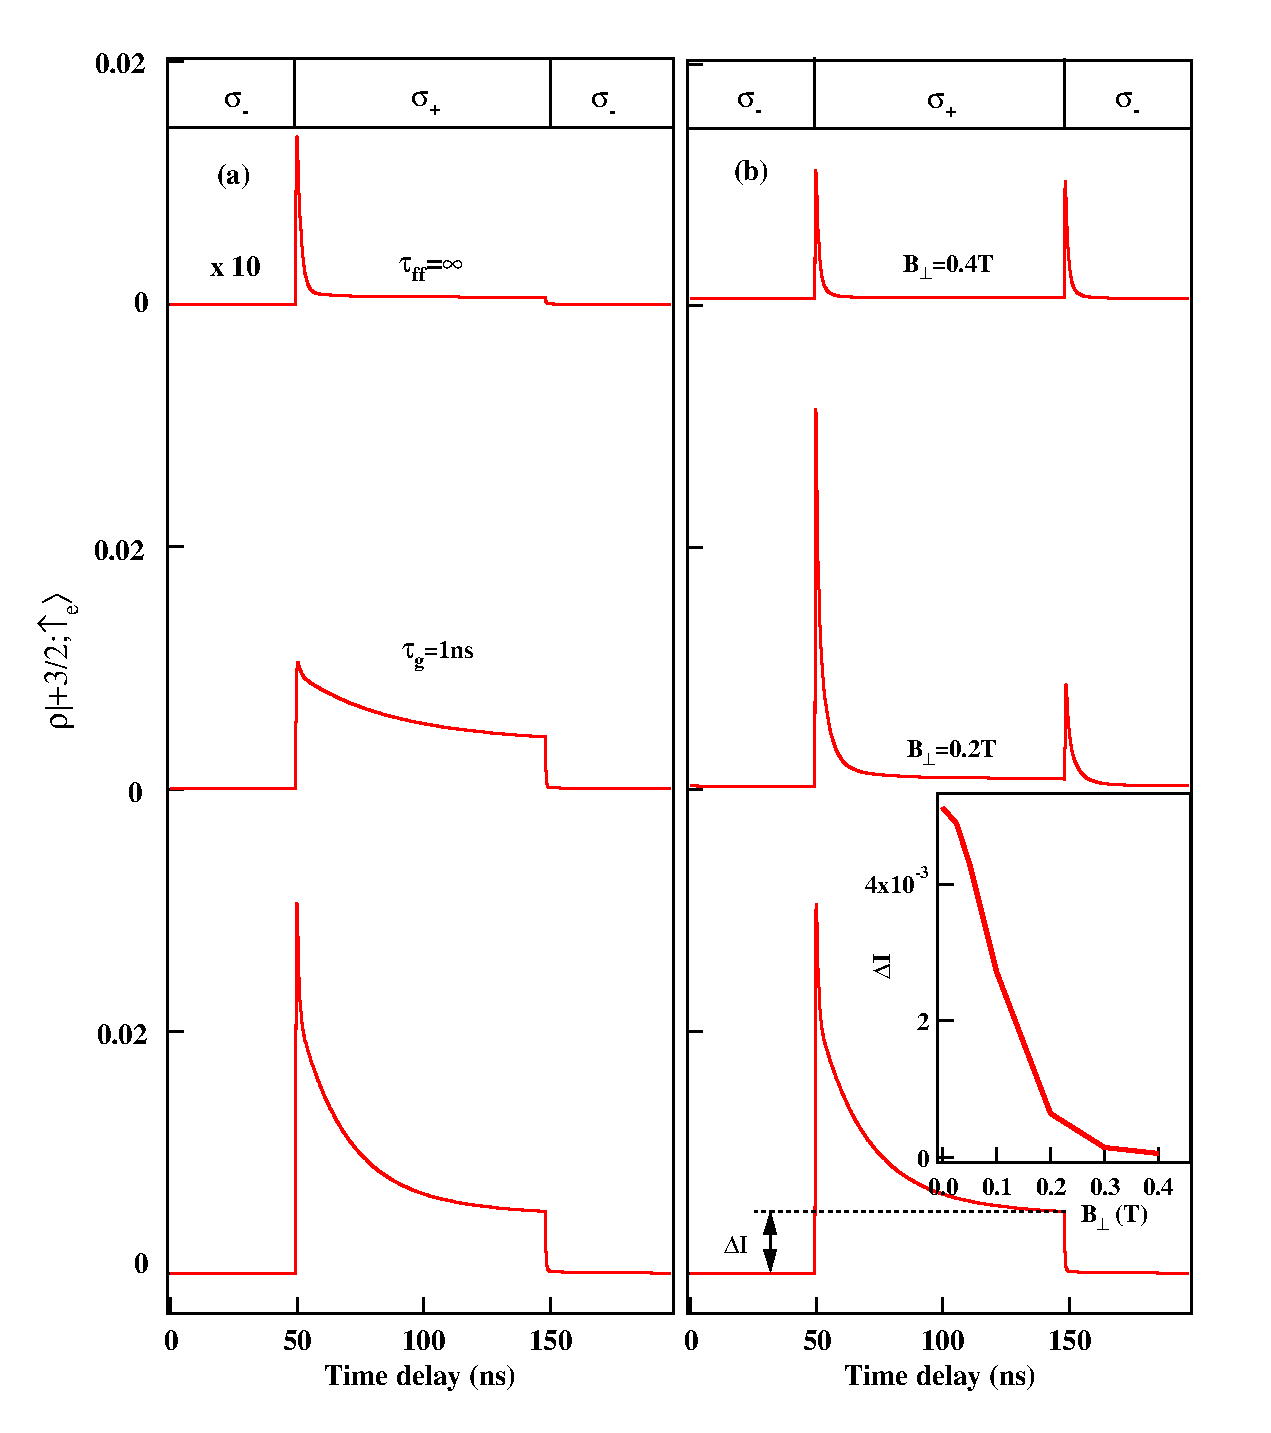
\includegraphics[width=3.3in]{Fig9.eps}
\caption{Resonant optical pumping transients detected in $\sigma-$ polarization under excitation with modulated circular polarization of $|3,+2\rangle$  and $|3,-2\rangle$  calculated with the QD parameters listed in table \ref{paraQD} and $\tau_r$=0.3ns, $\tau_{Mn}$=5 $\mu$s, $\tau_h$=10ns, $T_2^{hMn}$= 5 ns, $T_2^{eMn}$= 0.5 ns, $\tau_{ff}$=1.5 ns, T=10K and $\tau_g$=0.25ns. (a) Influence of a variation of $\tau_g$ and $\tau_{ff}$. (b) Influence of a transverse magnetic field $B_{\perp}$. The inset presents the magnetic field dependence of the difference of population for a $\sigma+$ or a $\sigma-$ excitation.}
\label{Fig9}
\end{figure}

The time evolution of $\rho_{|+\frac{3}{2};\uparrow_e\rangle}(t)$ normalized by $\rho_{|+\frac{3}{2};\uparrow_e\rangle}(\infty)$ and with the initial condition $\rho_{|+\frac{3}{2};\Uparrow_h\rangle}(0)=1$ (hole-Mn spin state $|+\frac{3}{2};\Uparrow_h\rangle$ just after the recombination of the exciton) accounts for the auto-correlation of the emission in $\sigma-$ polarization of the electron-Mn state $|3;+2\rangle$ under $cw$ resonant excitation. $\rho_{|+\frac{3}{2};\uparrow_e\rangle}(t)$ obtained with the QD parameters listed in table \ref{paraQD} is presented in Fig.~\ref{Fig8}(a). After a fast increase, the calculated population presents a maximum at short delay. With reasonable spin relaxation parameters (see caption of Fig.~\ref{Fig8}) the width and the amplitude of the maximum are in good agreement with the photon bunching signals observed experimentally.

The width of the bunching is controlled by all the spin-flips terms that can induce an escape out of the resonantly excited $\Lambda$ system. At zero transverse magnetic field, it is dominated by spin flips in the hole-Mn system. As illustrated in Fig.~\ref{Fig8}(a), suppressing $\tau_h$ gives a width of bunching controlled by the Hamiltonian evolution and decoherence larger than observed experimentally. The width could be further reduced by introducing an additional spin relaxation mechanism for the electron-Mn system.

The dependence on the excitation intensity, $\tau_g$, and transverse magnetic field, $B_{\perp}$, are also qualitatively well reproduced by the model (Fig.~\ref{Fig8}(c) and (d) respectively). At zero magnetic field, the leaks are dominated by $\tau_h$ and $\mathcal{H}_{eMn}$ induces fluctuations in a slightly longer time scale. The situation is different under a weak transverse magnetic field where the electron-Mn states are mixed introducing new channel of escape and significantly reducing the width of the bunching.

The presented model can qualitatively explain the observed behaviour of the autocorrelation signal with reasonable parameters. Given the large number of parameters, their values cannot be extracted precisely. Let us note however that suppressing the fast flip-flop process between the two hole-Mn ground states ($\tau_{ff}=\infty$ in Fig.~\ref{Fig8}(b)) still produce a bunching as a weak coherent transfer between the two ground states of the $\Lambda$ system still exist. With only this process, the calculated PL intensity is about 100 time smaller and the behaviour in transverse magnetic field is not compatible with the experimental results.

With this model, we can also calculate the population of the electron-Mn states under resonant excitation with alternated circular polarization and estimate the efficiency and dynamics of the optical pumping. Figure~\ref{Fig9} presents the calculated time evolution of the population of the electron-Mn state $|+\frac{3}{2},\Uparrow_h\rangle$ under excitation of $|3,+2\rangle$ in $\sigma+$ polarization or $|3,-2\rangle$ in $\sigma-$ polarization. This corresponds to the experimental configuration where the QD is resonantly excited with modulated circular polarization at the energy of $|3,+2\rangle$ and $|3,-2\rangle$ (absorption (2) in Fig.~\ref{Fig2}(b)) and the low energy resonant PL detected in $\sigma-$ polarisation. The main features of the time-resolved optical pumping experiments (see Fig.~\ref{Fig4} and Fig.~\ref{Fig5}) are well reproduced by the model. The timescale of the pumping transient, in the few tens of nanosecond range, and its excitation intensity dependence are in good agrement with the experiments (see figure~\ref{Fig9}(a)).

The influence of a transverse magnetic field, B$_{\perp}$, on the optical pumping transient can also be qualitatively described by this model. First, a significant reduction of the pumping time is observed for a weak magnetic field (B$_{\perp}$=0.2T in Fig.~\ref{Fig9}(b)). As for the autocorrelation, this acceleration is coming from the increase of the leakage out of the $\Lambda$ system induced by the mixing of the electron-Mn states. Secondly, the transients obtained when switching the polarization from $\sigma_{co}$ to $\sigma_{cross}$ and from $\sigma_{cross}$ to $\sigma_{co}$ become identical for B$_{\perp}\approx0.4$T, as observed in the experiments (Fig.~\ref{Fig5}(b)).

To understand this behaviour under B$_{\perp}$, let us remember that with $\sigma+$ light we resonantly excite $|3,+2\rangle$ from $|+\frac{5}{2},\Downarrow_h$ and excite $|3,-2\rangle$ from $|-\frac{5}{2},\Uparrow_h\rangle$ under $\sigma-$ excitation. In both cases we detect the population of $|+\frac{3}{2},\uparrow_e\rangle$ in $\sigma-$ polarization. If the states $|3,+2\rangle$ and $|3,-2\rangle$ are uncoupled, as it is the case at zero field, we do not detect any light during the $\sigma-$ excitation. With a sufficiently large mixing of $|3,+2\rangle$ and $|3,-2\rangle$ induced by the transverse magnetic field, for a $\sigma-$ excitation of $|3,-2\rangle$, the population can be coherently transferred to $|3,+2\rangle$ during the charged exciton lifetime and $\sigma-$ light is detected after a recombination towards $|+\frac{3}{2},\Uparrow_h\rangle$ \cite{Lafuente2015}. In the optical pumping sequence, we can then observe, in $\sigma-$ polarization, a transient when the $\sigma+$ excitation empties the state $|+\frac{5}{2},\Downarrow_h\rangle$ but also a similar transient when the $\sigma-$ excitation empties the state $|-\frac{5}{2},\Uparrow_h\rangle$. Let us note finally that, as expected, suppressing $\tau_{ff}$ from the model, a very weak average resonant PL and a fast optical pumping are obtained (Fig.~\ref{Fig9}(b), top curve).

\begin{figure}[hbt]
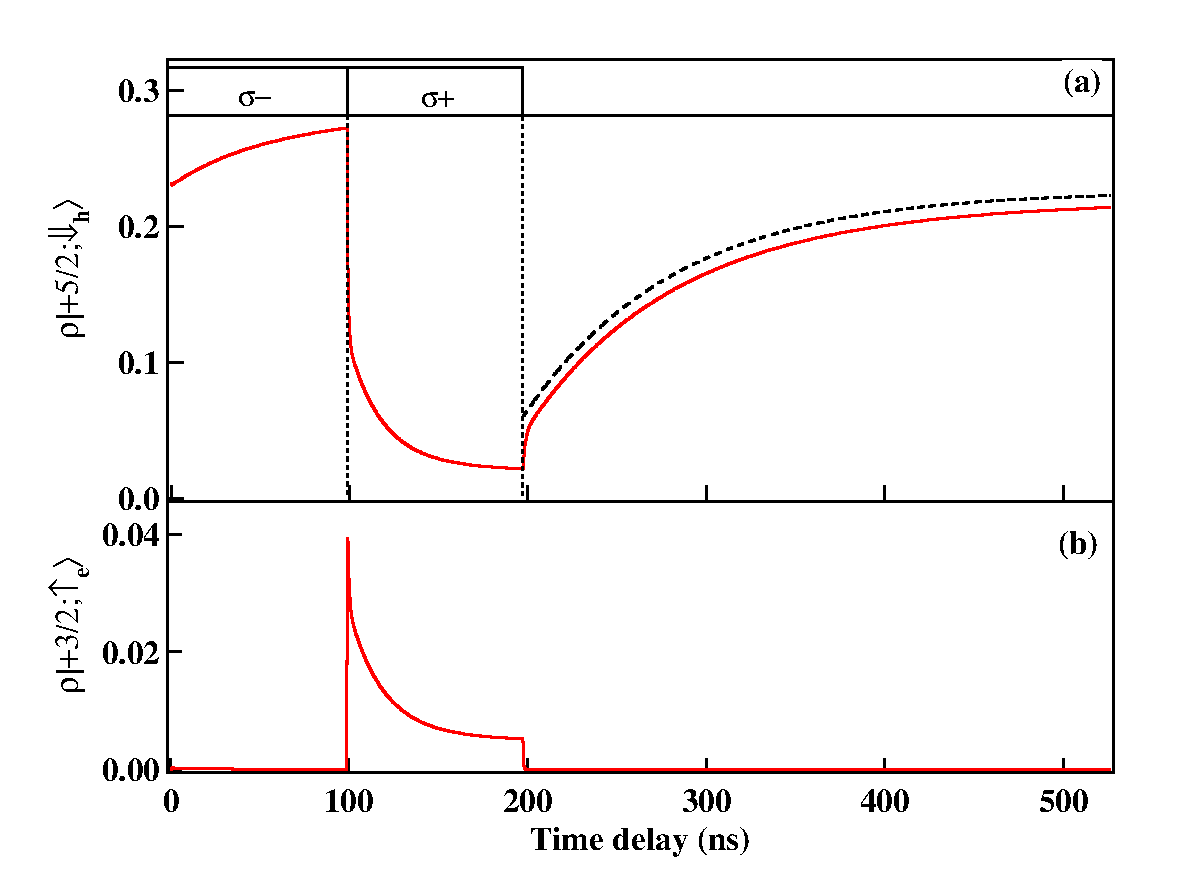
\includegraphics[width=3.3in]{Fig10.eps}
\caption{(a) Calculated time evolution in the dark of the population of the hole-Mn state $|+\frac{5}{2},\Downarrow_h\rangle$ initialized by a sequence of $\sigma-$/$\sigma+$ resonant excitation of $|3,-2\rangle$ and $|3,+2\rangle$. The dashed black line (shifted for clarity) is an exponential fit with a characteristic time $\tau_{relax}$=85 ns. (b) Corresponding calculated time evolution of the population $|+\frac{3}{2},\uparrow_e\rangle$.}
\label{Fig10}
\end{figure}

Including a dark time in the pumping sequence, we can also numerically evaluate the time required for the hole-Mn spin to return to the ground state of the excited $\Lambda$ system. The hole-Mn is first initialized under $cw$ circularly polarized excitation. The time evolution of the population of the state $|+5/2,\Downarrow_h\rangle$ prepared by a sequence of $\sigma-$/$\sigma+$ excitation resonant with $|3;+2\rangle$ (and $|3;-2\rangle$) is presented in Fig.\ref{Fig10}. When a the optical excitation is switched off, after an abrupt jump due to the optical recombination of the charge exciton, the ground hole-Mn state $|+5/2,\Downarrow_h\rangle$ is repopulated in a timescale of about 100 ns, much shorter than the Mn spin relaxation time used in the model. This relaxation is induced by the valence band mixing. In the presence of valence-band mixing, $\mathcal{H}_{hMn}^{ex}$ couples two by two the different hole-Mn levels. This coupling induces a transfer of population between the different hole-Mn levels. The transfer of population becomes irreversible in the presence of dephasing and controls to the hole-Mn spin relaxation.

\begin{figure}[hbt]
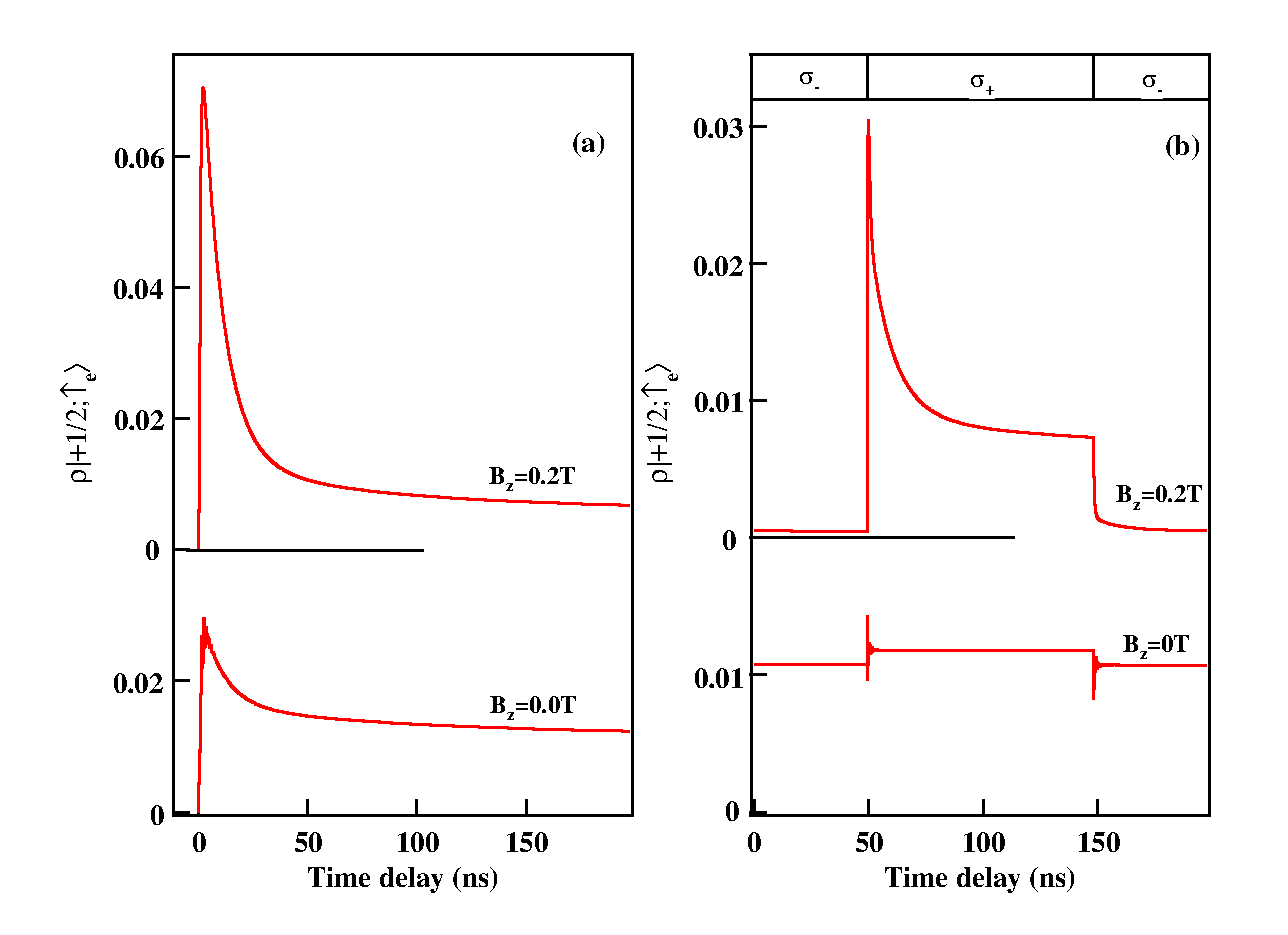
\includegraphics[width=3.3in]{Fig11.eps}
\caption{(a) Calculated time evolution of $\rho_{|+\frac{3}{2},\uparrow_e\rangle}(t)$ for a resonant excitation of $|3,+1\rangle$ and $|3,-1\rangle$ with the QD parameters listed in table \ref{paraQD} without and with a longitudinal magnetic field. (b) Corresponding calculated optical pumping transients under excitation with modulated circular polarization.}
\label{Fig11}
\end{figure}

The particular behaviour observed for a resonant excitation on (1) (Fig.~\ref{Fig2}(a) and Fig.~\ref{Fig4}(a)) is also explained by the developed model (see figure~\ref{Fig11}). The presence of a strain anisotropy term $E$ directly couples the electron-Mn states $|3,+1\rangle$ and $|3,-1\rangle$ \cite{Lafuente2015}. Under circularly polarized resonant excitation we either excite $|3,+1\rangle$ with $\sigma+$ photons or $|3,-1\rangle$ with $\sigma-$ photons. However, at zero magnetic field, the population is transferred between the two states in a time scale of a few hundreds picoseconds \cite{Lafuente2015}. Under a weak longitudinal magnetic field the Mn Zeeman energy dominates the strain anisotropy term and the coherent transfer is blocked. A large amplitude of bunching and an efficient optical pumping are restored. This behaviour observed in the experiments is qualitatively reproduced by the model.

The presented model explains the main behaviour of a positively charged Mn-doped QD under resonant optical excitation. It shows in particular the strong influence of the effective heavy-hole/light-hole splitting $\Delta_{lh}$ on the hole-Mn spin dynamics. The studied CdTe/ZnTe QDs have a weak valence band offset. The resulting small value of $\Delta_{lh}$ is first responsible for the large influence of the QDs' shape or strain anisotropy on the valence band mixing. The valence band mixing reduces the magnetic anisotropy of the hole-Mn system and its spin memory. A small $\Delta_{lh}$ also enhance the coupling of the hole-Mn spin with the strain field of acoustic phonons. This fast spin dynamics limits the use of such hybrid spin system in practical quantum information device. The use of different QD systems with a larger valence band offset and a larger heavy-hole/light-hole splitting would significantly slow down the hole-Mn spin relaxation \cite{Moehl2004}.


%The modelling also shows that a resonant excitation in a weak transverse magnetic field permits to efficiently prepare the hole-Mn spin in one of its ground state +1 or -1.


\section{Conclusion}

To conclude, using resonant PL of the positively charged exciton we have identified an efficient spin relaxation channel for coupled hole and Mn spins in a QD. A modelling confirms that hole-Mn flip-flops in a nanosecond timescale are induced by an interplay of hole-Mn exchange interaction and the lattice deformation of acoustic phonons. These flip-flops are responsible for the large PL intensity observed under resonant excitation of the $\Lambda$ systems present in positively charged Mn-doped QDs. We show that jumps out of an optically excited $\Lambda$ system are also possible. These leaks induce a large bunching of the resonant PL. They are also at the origin of the optical pumping of the coupled hole-Mn spins observed under circularly polarized resonant excitation. Escape out of the excited $\Lambda$ system can be enhanced by a transverse magnetic field which mixes electron-Mn states in the excited state of the charged QD. The fast hole-Mn spin dynamics revealed by these experiments make difficult the practical use of this hybrid spin for quantum information devices. However, the use of a different QD systems with a better hole confinement and a larger heavy-hole/light-hole spitting would significantly reduce the influence of valence band mixing on the hole-Mn spin relaxation and its interaction with acoustic phonons.


\begin{acknowledgements}

This work was realized in the framework of the Commissariat \`{a} l'Energie Atomique et aux Energies Alternatives (Institut Nanosciences et Cryog\'{e}nie) / Centre National de la Recherche Scientifique (Institut N\'{e}el) joint research team NanoPhysique et Semi-Conducteurs.

\end{acknowledgements}


\begin{appendix}

\section{Efficient hole-Mn flip-flops observed in neutral magnetic quantum dots.}

The mechanism of hole-Mn flip-flop evidenced and modelled in the case of positively charged magnetic QDs can also be directly observed in the resonant PL of neutral QDs. This is illustrated in Fig.~\ref{FigAppendix} which presents the PL of the exciton in a QD where all the dark states are well separated from the bright states and can be observed at zero magnetic field on the low energy side of the spectra.

\begin{figure}[hbt]
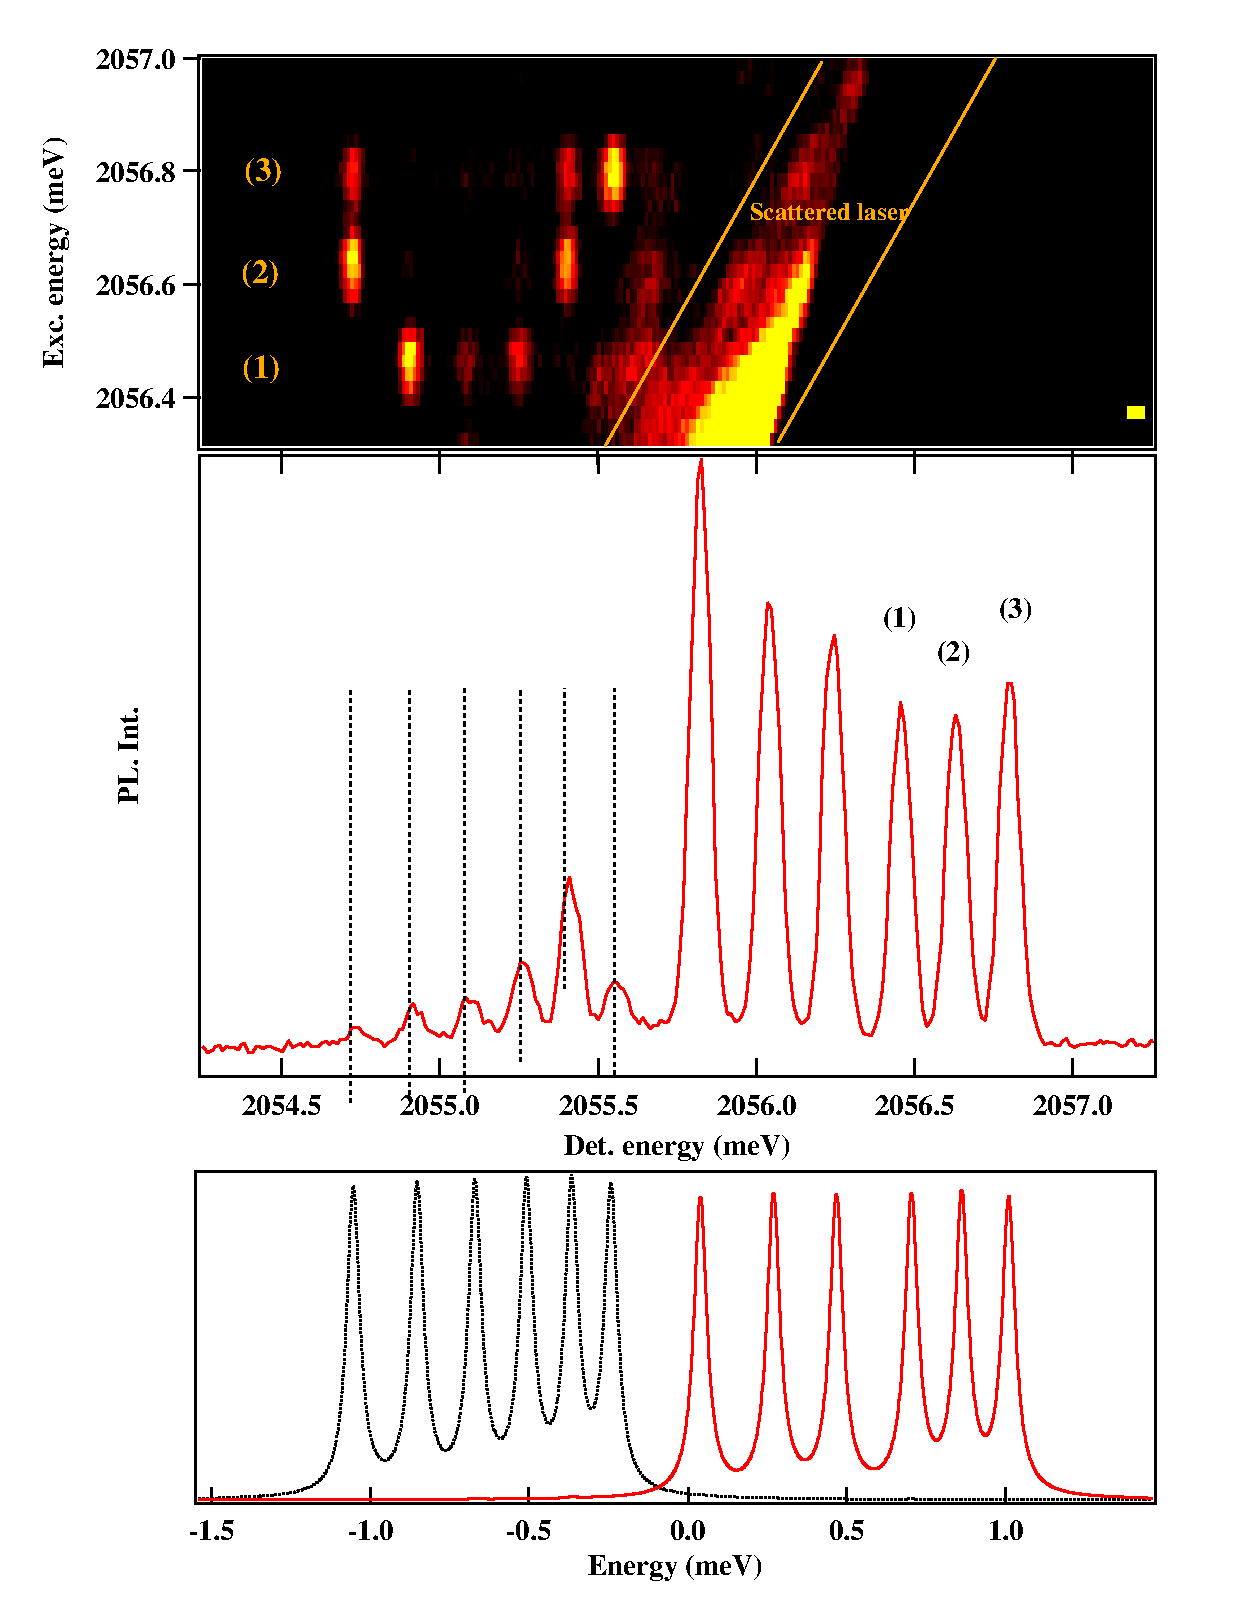
\includegraphics[width=3.3in]{FigAppendix.eps}
\caption{PL intensity map detected on the dark states of a Mn-doped QD. The excitation laser is scanned across the three high energy bright states. Excitation and detection are circularly cross-polarized. The resonances (1-3) are discussed in the text. The bottom panel presents calculated bright $|+1\rangle$ (plain line) and dark $|-2\rangle$ (dotted line) energy levels with $I_{eMn}$=-0.03 meV, $I_{hMn}$=0.12 meV, $I_{eh}$=-0.78 meV, $\rho_s/\Delta_{lh}=0.05$ and $\eta$=10$\mu$eV.}
\label{FigAppendix}
\end{figure}

In the PL excitation experiments presented in Fig.~\ref{FigAppendix}, the detection window is set on the dark states while a circularly cross-polarized laser is scanned on the three high energy levels of the bright exciton. Three successive resonances are observed.

(1): An excitation on $|+1,S_z=+1/2\rangle$ produces the dominant PL on a dark states associated with a Mn spin state $\pm3/2$. As a Mn spin flip by two units is unlikely, we then attribute this PL to $|-2,S_z=+3/2\rangle$. The transfer between these states involves a hole-Mn flip-flop. The second contribution comes from the state $|+2,S_z=+1/2\rangle$. It corresponds to a transfer conserving the Mn spin and involving a spin flip of the electron.

(2): An excitation on $|+1,S_z=+3/2\rangle$ produces the dominant PL on a dark states associated with a Mn spin state $\pm5/2$. As discussed above, a Mn spin flip by four units is unlikely, we then attribute this PL to $|-2,S_z=+5/2\rangle$. The transfer involve a hole-Mn flip-flop. The second contribution comes from the state $|+2,S_z=+3/2\rangle$. It corresponds to a conservation of the Mn spin and a spin flip of the electron.

(3): From an excitation on $|+1,S_z=+5/2\rangle$, the dominant PL comes from the state $|+2,S_z=+5/2\rangle$. It corresponds to a transfer with conservation of the Mn spin and a spin flip of the electron. A weaker PL is also observed from $|-2,S_z=+5/2\rangle$ after a spin flip of the hole and from $|+2,S_z=+3/2\rangle$. The latter transfer involves an electron-Mn flip-flop. Let's note that in the state $|+1,S_z=+5/2\rangle$ a hole-Mn flip-flop is forbidden (parallel hole and Mn spin).

If we resume the observed resonances in this QD, we can distinguish two types of spin transfer which occurs within the lifetime of the exciton:
\begin{itemize}
\item An efficient transfer from a bright to a dark state involving a
hole-Mn flip-flop. This produces a change of one unit of the Mn spin state.
\item Transfer from a bright to a dark state involving a
carrier spin-flip and conservation of the Mn spin. Electron
spin flips are the most efficient in QD with a weak valence
band mixing (case of QD presented in
Fig.~\ref{FigAppendix}).
\end{itemize}

\end{appendix}




\begin{thebibliography}{}

\bibitem{Petta2005} J. R. Petta, A. C. Johnson, J. M. Taylor, E. A. Laird, A. Yacoby, M. D. Lukin, C. M. Marcus, M. P. Hanson, A. C. Gossard, Science {\bf 309}, 2180 (2005).
\bibitem{Veldhorst2015} M. Veldhorst, C. H. Yang, J. C. C. Hwang, W. Huang, J. P. Dehollain, J. T.Muhonen, S. Simmons,A. Laucht, F. E. Hudson, K. M. Itoh, A. Morello, A. S. Dzurak, Nature (London) {\bf 526}, 410 (2015).
\bibitem{Koenrad2011} P. M. Koenraad, M. E. Flatte, Nat. Mater. {\bf 10}, 91 (2011).
\bibitem{Atature2006} M. Atature, J. Dreiser, A. Badolato, A. Hogele, K. Karrai, A. Imamoglu, Science {\bf 312}, 551 (2006).
\bibitem{Press2008} D. Press, T. D. Ladd, B. Zhang, and Y. Yamamoto, Nature (London) {\bf 456}, 218 (2008).
\bibitem{Gerardot2008} B. D. Gerardot, D. Brunner, P. A. Dalgarno, P. Ohberg, S. Seidl, M. Kroner, K. Karrai, N. G. Stoltz, P. M. Petroff, R. J. Warburton, Nature (London) {\bf 451}, 441 (2008).
\bibitem{DeGreve2011} K. De Greve, P. L. McMahon, D Press, T. D. Ladd, D. Bisping, C. Schneider, M. Kamp, L. Worschech, S. Hofling, A. Forchel, Y. Yamamoto, Nat. Phys. {\bf 7}, 872 (2011).

\bibitem{Besombes2004} L. Besombes, Y. Leger, L. Maingault, D. Ferrand, H. Mariette, J. Cibert, Phys. Rev. Lett. {\bf 93}, 207403 (2004).
\bibitem{LeGall2011} C. Le Gall, A. Brunetti, H. Boukari, L. Besombes, Phys. Rev. Lett. {\bf 107}, 057401 (2011).
\bibitem{Kudelski2007} A. Kudelski, A. Lemaitre, A. Miard, P. Voisin, T.C.M. Graham, R.J. Warburton, O. Krebs, Phys. Rev. Lett. {\bf 99}, 247209 (2007).
\bibitem{Kobak2014} J. Kobak, T. Smolenski, M. Goryca, M. Papaj, K. Gietka, A. Bogucki, M. Koperski, J.-G. Rousset, J. Suffczynski, E. Janik, M. Nawrocki, A. Golnik, P. Kossacki, W. Pacuski, Nature Com. {\bf 5}, 3191(2014).
\bibitem{Besombes2012} L. Besombes, C.L. Cao, S. Jamet, H. Boukari, J. Fernandez-Rossier, Phys. Rev. B  {\bf 86}, 165306 (2012).
\bibitem{Krebs2013} O. Krebs, A. Lemaitre, Phys. Rev. Lett. {\bf 111}, 187401 (2013).
\bibitem{Besombes2015} L. Besombes, H. Boukari, C. Le Gall, A. Brunetti, C.L. Cao, S. Jamet, B. Varghese, Nanophotonics {\bf 4}, p.75 (2015).
\bibitem{Reiter2013} D. E. Reiter, V. M. Axt, T. Kuhn, Phys. Rev. B {\bf 87}, 115430 (2013).
\bibitem{Goryca2009} M. Goryca, T. Kazimierczuk, M. Nawrocki, A. Golnik, J. A. Gaj, P. Kossacki, P. Wojnar, G. Karczewski, Phys. Rev. Lett. {\bf 103}, 087401 (2009).
\bibitem{Oberg2014} J. C. Oberg, M. Reyes Calvo, F. Delgado, M. Moro-Lagares, D. Serrate, D. Jacob, J. Fernandez-Rossier, C. F. Hirjibehedin, Nat. Nanotechnol. 9, 64 (2014) and references therein.

\bibitem{Leger2005} Y. Leger, L. Besombes, L. Maingault, D. Ferrand, H. Mariette Phys. Rev. B 72, 241309(R) (2005).
\bibitem{Vyborny2012} K. Vyborny, J. E. Han, R. Oszwaldowski, I. Zutic, and A. G.Petukhov, Phys. Rev. B 85, 155312 (2012).
\bibitem{Varghese2014} B. Varghese, H. Boukari, L. Besombes, Phys. Rev. B {\bf 90}, 115307 (2014).
\bibitem{Lafuente2015} A. Lafuente-Sampietro, H. Boukari, L. Besombes, Phys. Rev. B {\bf 92}, 081305(R) (2015).
\bibitem{Houel2014} J. Houel, J. H. Prechtel, A. V. Kuhlmann, D. Brunner, C. E. Kuklewicz, B. D. Gerardot, N. G. Stoltz, P. M. Petroff, R. J. Warburton, Phys. Rev. Lett. {\bf 112}, 107401 (2014).

\bibitem{Wojnar2011} P. Wojnar, C. Bougerol, E. Bellet-Amalric, L. Besombes, H. Mariette, H. Boukari, Journal of Crystal Growth {\bf 335}, 28 (2011).
\bibitem{LeGall2010} C. Le Gall, R. S. Kolodka, C. L. Cao, H. Boukari, H. Mariette, J. Fernandez-Rossier, L. Besombes, Phys. Rev. B {\bf 81}, 245315 (2010).

\bibitem{LeGall2009} C. Le Gall, L. Besombes, H. Boukari, R. Kolodka, J. Cibert, H. Mariette, Phys. Rev. Lett. {\bf 102}, 127402 (2009).
\bibitem{Goryca2014} M. Goryca, M. Koperski, P. Wojnar, T. Smoleński, T. Kazimierczuk, A. Golnik, P. Kossacki, Phys. Rev. Lett. {\bf 113}, 227202 (2014).
\bibitem{Qazzaz1995} M. Qazzaz, G. Yang, S.H. Xin, L. Montes, H. Luo, J.K. Furdyna, Solid State Communications {\bf 96}, 405 (1995).
\bibitem{Causa1980} M.T. Causa, M. Tovar, S.B. Oseroff, R. Calvo, W. Giriat, Phys. Lett. {\bf A77}, 473 (1980).
\bibitem{Trojnar2013} A. H. Trojnar, M. Korkusinski, U. C. Mendes, M. Goryca, M. Koperski, T. Smolenski, P. Kossacki, P. Wojnar, P. Hawrylak, Phys. Rev. B {\bf 87}, 205311 (2013).
\bibitem{Besombes2014} L. Besombes, H. Boukari, Phys. Rev. B {\bf 89}, 085315 (2014).
\bibitem{Jamet2013} S. Jamet, H. Boukari, L. Besombes, Phys. Rev. B {\bf 87}, 245306 (2013).
\bibitem{Fernandez2006} J. Fernandez-Rossier, Phys. Rev. B {\bf 73}, 045301 (2006).
\bibitem{Leger2007} Y. Leger, L. Besombes, L. Maingault, H. Mariette, Phys. Rev. B {\bf 76}, 045331 (2007).
\bibitem{Besombes2005} L. Besombes, Y. Leger, L. Maingault, D. Ferrand, H. Mariette, J. Cibert, Phys. Rev. B {\bf 71}, 161307(R) (2005).

\bibitem{Besombes2001} L. Besombes, K. Kheng, L. Marsal, H. Mariette, Phys. Rev. B {\bf 63}, 155307 (2001).
\bibitem{Cohen} C. Cohen-Tannoudji, B. Diu, F. Laloe, {\it Mecanique quantique} (Hermann, Paris, 1973).
\bibitem{Tsitsishvili2003} E. Tsitsishvili, R. V. Baltz, H. Kalt, Phys. Rev. B {\bf 67}, 205330 (2003).
\bibitem{Roszak2007} K. Roszak, V.M. Axt, T. Kuhn, P. Machnikowski, Phys. Rev. B {\bf 76}, 195324 (2007).
\bibitem{Mahan} G.D. Mahan, {\it Many-Particle Physics} (Plenum Press, New York, 1993).
\bibitem{Woods2004} L.M. Woods, T.L. Reinecke, R. Kotlyar, Phys. Rev. B {\bf 69}, 125330 (2004).

\bibitem{Adachi2005} S. Adachi, {\it Properties of group IV, III-V and II-VI semiconductors} (John Wiley and Sons Ltd, 2005).
\bibitem{Michler2003} P. Michler, {\it Single quantum dots fundamentals, applications and new concepts} (Springer, Berlin, 2003).
\bibitem{Bester2015} J-W. Luo, G. Bester, A. Zunger, Phys. Rev. B {\bf 92}, 165301 (2015).

\bibitem{Exter2009} M.P. van Exter, J. Gudat, G. Nienhuis, D. Bouwmeester, Phys. Rev. A {\bf 80}, 023812 (2009).
\bibitem{Roy2011} C. Roy and S. Hughes, Phys. Rev. X {\bf 1}, 021009 (2011).
\bibitem{Cao2011} C. L. Cao, L. Besombes, J. Fernandez-Rossier, Phys. Rev. B {\bf 84}, 205305 (2011).
\bibitem{Cywinski2010} L. Cywinski, Phys. Rev. B {\bf 82}, 075321 (2010).
\bibitem{LeGall2012} C. Le Gall, A. Brunetti, H. Boukari, L. Besombes, Phys. Rev. B {\bf 85}, 195312 (2012).
\bibitem{Govorov2005} A. O. Govorov, A. V. Kalameitsev, Phys. Rev. B {\bf 71}, 035338 (2005).
\bibitem{Moehl2004} S. Moehl, F. Tinjod, K. Kheng, H. Mariette, Phys . Rev. B {\bf 69}, 245318 (2004).

\end{thebibliography}


\end{document}
